\documentclass[a4paper,11pt]{jreport}

\setcounter{tocdepth}{3}
\setcounter{page}{-1}

\setlength{\oddsidemargin}{0.1in}
\setlength{\evensidemargin}{0.1in}
\setlength{\topmargin}{0in}
\setlength{\textwidth}{6in}
% \setlength{\textheight}{10.1in}
\setlength{\parskip}{0em}
\setlength{\topsep}{0em}

\renewcommand{\baselinestretch}{1.1}

% \newcommand{\zu}[1]{{\gt \bf 図\ref{#1}}}

%% タイトル生成用パッケージ(重要)
\usepackage{sie-jp-utf8}

\usepackage[dvipdfmx]{graphicx,color}

\usepackage{theorem}
\usepackage{amsmath,amssymb}
\usepackage{ascmac}
\usepackage{mathtools}
\usepackage{proof}
\usepackage{stmaryrd}
\usepackage{listings,jlisting}
\usepackage{here}
\usepackage{verbatim}
\usepackage{framed}
\usepackage{algorithm}
\usepackage{algpseudocode}


\lstset{
  basicstyle=\ttfamily,
  columns=fullflexible,
  keepspaces=true,
}

\newenvironment{vq}
{%begin
  \VerbatimEnvironment \begin{screen} \begin{quote} \begin{Verbatim}
      }
      {%end
      \end{Verbatim} \end{quote} \end{screen}
}
\newtheorem{theorem}{theorem}[section]

\definecolor{DarkGreen}{rgb}{0,0.5,0}
\definecolor{Magenta}{rgb}{1.0, 0.0, 1.0}

\newcommand\cbra{\texttt{<}}
\newcommand\cket{\texttt{>}}

\newcommand\lam{\lambda}

\newcommand\codeTs[2]{\langle{#1}\rangle{\textbf{\textasciicircum}{#2}}}

\newcommand\fordo[2]{\textbf{for}~{#1}~\textbf{to}~{#2}~\textbf{do}}
\newcommand\cfordo[2]{\underline{\textbf{for}}~{#1}~\underline{\textbf{to}}~{#2}~\underline{\textbf{do}}}
\newcommand\cfor[1]{\underline{\textbf{for}}~{#1}}

\newcommand\too{\leadsto^*}
\newcommand\downtoo{\rotatebox{-90}{$\leadsto^*$}}
\newcommand\pink[1]{\textcolor{pink}{#1}}
\newcommand\red[1]{\textcolor{red}{#1}}
\newcommand\green[1]{\textcolor{green}{#1}}
\newcommand\magenta[1]{\textcolor{magenta}{#1}}
\newcommand\blue[1]{\textcolor{blue}{#1}}

\newcommand\fun[2]{\lambda{#1}.{#2}}

\newcommand\Resetz{\textbf{reset0}}
\newcommand\Shiftz{\textbf{shift0}}
\newcommand\Throw{\textbf{throw}}
\newcommand\resetz[1]{\Resetz~{#1}}
\newcommand\shiftz[2]{\Shiftz~{#1}\to{#2}}
\newcommand\throw[2]{\Throw~{#1}~{#2}}

\newcommand\cfun[2]{\underline{\lambda}{#1}.{#2}}
\newcommand\ccfun[2]{\underline{\underline{\lambda}}{#1}.{#2}}

\newcommand\cResetz{\underline{\textbf{reset0}}}
\newcommand\cShiftz{\underline{\textbf{shift0}}}
\newcommand\cThrow{\underline{\textbf{throw}}}
\newcommand\cresetz[1]{\cResetz~{#1}}
\newcommand\cshiftz[2]{\cShiftz~{#1}\to{#2}}
\newcommand\cthrow[2]{\cThrow~{#1}~{#2}}

\newcommand\cPlus{\underline{\textbf{+}}}
\newcommand\Plus{\textbf{+}}

\newcommand\cLet{\underline{\textbf{let}}}
\newcommand\cIn{\underline{\textbf{in}}}
\newcommand\clet[3]{\cLet~{#1}={#2}~\cIn~{#3}}
\newcommand\csp[1]{\texttt{\%}{#1}}
\newcommand\cint{\underline{\textbf{int}}}
\newcommand\code[1]{\texttt{<}{#1}\texttt{>}}
\newcommand\codebegin{\texttt{<}}
\newcommand\codeend{\texttt{>}}

\newcommand\intT{\mbox{\texttt{int}}}
\newcommand\boolT{\mbox{\texttt{bool}}}

\newcommand\codeT[2]{\langle{#1}\rangle^{#2}}
\newcommand\funT[3]{{#1} \stackrel{#3}{\rightarrow} {#2}}
\newcommand\contT[3]{{#1} \stackrel{#3}{\Rightarrow} {#2}}

\newcommand\ord{\ge}

\newcommand\Let{\textbf{let}}
\newcommand\In{\textbf{in}}
\newcommand\letin[3]{\Let~{#1}={#2}~\In~{#3}}

\newcommand\iif{\textbf{if}}
\newcommand\then{\textbf{then}}
\newcommand\eelse{\textbf{else}}
\newcommand\ift[3]{\textbf{if}~{#1}~\textbf{then}~{#2}~\textbf{else}~{#3}}
\newcommand\cif[3]{\underline{\textbf{if}}~\code{{#1}}~\code{{#2}}~\code{{#3}}}
\newcommand\cIf{\underline{\textbf{if}}}

\newcommand\fix{\textbf{fix}}
\newcommand\cfix{\underline{\textbf{fix}}}

\newcommand\lto{\leadsto}
\newcommand\cat{~\underline{@}~}

\newcommand\ksubst[2]{\{{#1}\Leftarrow{#2}\}}

\newcommand\cFor{\underline{\textbf{for}}}
\newcommand\forin[2]{\textbf{for}~{#1}~\textbf{to}~{#2}~\textbf{do}}
\newcommand\cforin[2]{\underline{\textbf{for}}~{#1}~\underline{\textbf{to}}~{#2}~\underline{\textbf{do}}}
\newcommand\cArray[1]{\underline{[{#1}]}}
\newcommand\cArrays[2]{\underline{[{#1}][{#2}]}}
\newcommand\aryset[3]{{#1}[{#2}]\leftarrow {#3}}
\newcommand\caryset[3]{\underline{\textbf{aryset}}~{#1}~{#2}~{#3}}
\newcommand\set{\underline{\textbf{set}}}

% コメントマクロ
\newcommand\kam[1]{\red{kam said: {#1}}}
\newcommand\oishi[1]{\blue{oishi said: {#1}}}

\theoremstyle{break}

\newtheorem{theo}{定理}[section]
\newtheorem{defi}{定義}[section]
\newtheorem{lemm}{補題}[section]

\algnewcommand\algorithmicforeach{\textbf{for each}}
\algdef{S}[FOR]{ForEach}[1]{\algorithmicforeach\ #1\ \algorithmicdo}

\renewcommand{\topfraction}{.85}
\renewcommand{\bottomfraction}{.60}
\renewcommand{\textfraction}{.15}
\renewcommand{\floatpagefraction}{.6}

\newcommand\smallerscope[2]{#1 \ord #2}
\newcommand\greaterscope[2]{#2 \ord #1}
\newcommand\longer[2]{{#1} \ord {#2}}
% \newcommand*\defeq{\stackrel{\text{def}}{=}}
\newcommand\Int{\mbox{\texttt{Int}}}
\newcommand\Bool{\mbox{\texttt{Bool}}}

\newcommand\uni{\cup} % !!! 現在の順序では「∪」

%% タイトル
%% 【注意】タイトルの最後に\\ を入れるとエラーになります
\title{安全なコード移動が可能なコード生成言語の\\型システムの設計と実装}

%% 著者
\author{大石 純平}
%% 学位 (2012/11 追加)
\degree{修士(工学)}
%% 指導教員
\advisor{亀山 幸義}

%% 専攻名 と 年月
%% 年月は必要に応じて書き替えてください。
\majorfield{コンピュータサイエンス} \yearandmonth{2017年 3月}

\begin{document}
\maketitle
\thispagestyle{empty}
\newpage

\thispagestyle{empty}
\vspace*{20pt plus 1fil}
\parindent=1zw
\noindent
%%
%% 論文の概要(Abstract)
%%
\begin{center}
  {\bf 概要}
  \vspace{5mm}
\end{center}
コード生成法は,プログラムの実行性能の高さと保守性・再利用性を両立でき
るプログラミング手法として有力なものである.本研究は,コード生成法で必
要とされる多段階let挿入等を簡潔に表現できるコントロールオペレータ
である shift0/reset0を持つコード生成言語とその型システムを構築し,
生成されたコードの型安全性を保証するための型システムを構築した.多段階let挿入は,入れ子になった
forループを飛び越えたコード移動を許す仕組みであり,ループ不変式の移動
などのために必要である.コード生成言語の型安全性に関して,破壊的代入
を持つ体系に対する須藤らの研究等があるが,本研究は,彼らの環境識別子
にジョインを追加するという拡張により,shift0/reset0 を持つコード生成言
語に対する型システムが構築できることを示した.

%%%%%
\par
\vspace{0pt plus 1fil}
\newpage

\pagenumbering{roman} % I, II, III, IV
\tableofcontents
\listoffigures
% \listoftables

\pagebreak \setcounter{page}{1}
\pagenumbering{arabic} % 1,2,3

\chapter{はじめに}
コード生成法は,プログラムの生産性・保守性と実行性能の高さを両立させら
れるプログラミング手法として有力なものである.
本研究は,コード生成法で必要とされる「多段階let挿入」等を簡潔に表現で
きるコントロールオペレータである shift0/reset0を持つコード生成言語とそ
の型システムを構築し,生成されたコードの型安全性を静的に保証する言語体
系および型システムを設計する.
これにより,コード生成器のコンパイル段階,すなわち,実際にコードが生成
されてコンパイルされるより遥かに前の段階でのエラーの検出が可能となると
いう利点がある.

コード生成におけるlet挿入は,生成されたコードを移動して効率良いコード
に変形するための機能であり,ループ不変式をforループの外側に移動したり,
コードの計算結果を共有するなどのコード変換(コード最適化)において必要な機能である.
多段階let挿入は,入れ子になったforループ等を飛び越えて,コードを移動す
る機能である.

ここでいう安全性は,構文的に正しいプログラムであること,
文字列同士の加算や乗算を決して行わない等の通常の型安全性を満たすことのほか,
自由変数やプログラム特化後において利用できない変数に依存したプログラム
を生成しないという,変数や変数スコープに関する性質を含む概念である.

この研究での大きな課題は,従来のコード生成のためのプログラミング言語の多くが,純粋なラムダ計算に基づく関数型プログラミング言語を基礎としており,効率の良いコードを生成する多くの技法をカバーしていないことである.これを克服する体系,すなわち,効率良いプログラムを記述するための表現力を高めつつ,安全性が保証された体系が求められている.

本研究は,
多段階let挿入を可能とするコード生成体系の構築のため,
比較的最近になって理論的性質が解明されたshift0/reset0\cite{Materzok2011} という
コントロールオペレータに着目する.
このコントロールオペレータに対する型規則を適切に設計することにより,
型安全性を解決することを目的とする.
コントロールオペレータを含む項の計算について分析した結果,
スコープの包含関係が逆転することや2つのスコープの合流があることから,
変数スコープを表す識別子にジョイン(和集合)を追加すればよいという着想を
得て,型システムを設計することに成功した.

本研究に関連した従来研究としては,
束縛子を越えない範囲でのコントロールオペレータを許した研究や,
局所的な代入可能変数を持つ体系に対する須藤らの研究\cite{Sudo2014},
後者を,グローバルな代入可能変数を持つ体系に拡張した研究
\cite{Aplas2016}などがある.
しかし,いずれの研究でも 多段階のforループを飛び越えたlet挿入は許していない.
本研究は,須藤らの研究をベースに,
shift0/reset0 を持つコード生成体系を設計した点に新規性がある.

%%% Local Variables:
%%% mode: japanese-latex
%%% TeX-master: "master_oishi"
%%% End:

\section{準備}

\subsection{コード生成の例}
\begin{frame}
  \frametitle{コード生成言語による記述例}

  \begin{align*}
    \visible<1->{\text{コード生成器}} \visible<1->{&\phantom{\too} \text{生成されるコード}} \\
    \visible<1->{(\cint~ 3)} \visible<1->{&\too \code{3}} \\
    \visible<1->{(\cint~ 3)~ \cPlus~ (\cint~ 5)} \visible<1->{&\too \code{3 + 5}} \\
    \visible<1->{\cfun{x}{~(x~ \cPlus~ (\cint~ 3))}} \visible<1->{&\too \code{\fun{x'}{~(x' + 3)}}} \\
    \visible<1->{\cfordo{x = \cdots}{\cdots}~ \cdots}
    \visible<1->{&\too \code{\fordo{x' = \cdots}{\cdots}~ \cdots}}
  \end{align*}

  % \begin{visibleenv}<2>
  %   \begin{exampleblock}{コードコンビネータ}
  %     \begin{itemize}
  %     \item 下線つきの演算子
  %     \item コードを引数にとり,コードを返す
  %     \end{itemize}
  %   \end{exampleblock}
  % \end{visibleenv}

\end{frame}

\subsection{コード生成器と生成されるコード}

\begin{frame}
  \frametitle{let挿入(コード移動)の実現方法}

  \begin{visibleenv}<1->
    \begin{columns}
      \begin{column}{0.5\textwidth}%% [横幅] 0.2\textwidth = ページ幅の 20 %
        コード生成器
        \begin{align*}
          & ~ \cfordo{x = e1}{e2} \\
          & ~~~ \cfordo{y = e3}{e4} \\
          & ~~~~~~\caryset{\code{a}}{(x,y)}~ ~ \\
          & ~~~~~~~~\magenta{\cLet ~u ~= ~\text{cc} ~\cIn}~~ \text{u}
        \end{align*}
      \end{column}
      $\too$
      \begin{column}{0.5\textwidth}%% [横幅] 0.2\textwidth = ページ幅の 20 %
        生成したいコード
        \begin{align*}
          & \cbra \fordo{x' = e1'}{e2'} \\
          & ~~\magenta{\Let ~u' ~= ~\text{cc}' ~\In} \\
          & ~~~~\fordo{y' = e3'}{e4'} \\
          & ~~~~~~\aryset{a}{x',y'}{u'} \cket
        \end{align*}
      \end{column}
    \end{columns}
  \end{visibleenv}

  \begin{visibleenv}<2>
    \begin{exampleblock}{shift0/reset0の導入}
      \red{shift0/reset0} 等を用いることで,(多段階)let挿入等を行う
    \end{exampleblock}
  \end{visibleenv}
\end{frame}

% \subsection{多段階let 挿入}

% \begin{frame}
%   \frametitle{shift0/reset0 によるlet挿入}
%   \noindent
%   \begin{align*}
%     \uncover<3->{\Resetz ~(E[\Shiftz~ k \to e]) ~\leadsto~ e \ksubst{k}{E}}
%   \end{align*}

%   \noindent

%   %   \begin{align*}
%   %     \text{コード生成器:}~~
%   %     & \uncover<4->{\blue{\Resetz}} ~~\cfordo{x = e1}{e2} \\
%   %     & ~~\uncover<2-3>{\blue{\Resetz}} ~~\cfordo{y = e3}{e4} \\
%   %     & ~~~~\uncover<2->{\blue{\Shiftz}~\blue{k}~\to}~
%   %     \magenta{\cLet~u=t~\cIn} \\
%   %     & ~~~~~~\uncover<2->{(\blue{\Throw~k}}~(\caryset{a}{(x,y)}{u})
%   %     \uncover<2->{)} \\
%   %     &   \uncover<3,5->{\blue{k}}
%   %     \only<3>{\Leftarrow ~~\cfordo{y = e3}{e4}~[\ ]}
%   %     \only<5->{\Leftarrow ~~\cfordo{x = e1}{e2} ~~\cfordo{y = e3}{e4} ~~[\ ]} \\
%   %     \text{生成コード:}~~
%   %     & \uncover<3,5->{\cbra~}
%   %     \only<3>{\fordo{x' = e1'}{e2'}} \only<5->{\magenta{\Let ~u' ~= ~t' ~\In}} \\
%   %     & ~~
%   %     \only<3>{\magenta{\Let ~u' ~= ~t' ~\In}} \only<5->{\fordo{x' = e1'}{e2'}} \\
%   %     & ~~~~\uncover<3,5->{\fordo{y' = e3'}{e4'}} \\
%   %     & ~~~~~~\uncover<3,5->{\aryset{a}{x',y'}{u'} ~\cket}
%   %   \end{align*}

%   \begin{align*}
%     \scriptsize{\text{コード生成器:}}~~
%     & \uncover<2-3>{\blue{\Resetz}} \only<1-2>{~\cfordo{x = e1}{e2}} \uncover<3>{\green{~\cfordo{x = e1}{e2}}}\\
%     & ~~~~~~~~~~~ \only<1-2>{\cfordo{y = e3}{e4}} \uncover<3>{\green{\cfordo{y = e3}{e4}}}\\
%     & ~~~~~~~~~~~~ \only<1-2>{\set~a~(x,y)~} \only<3>{\green{\set~a~(x,y)}~} \only<4->{~~~~~~~~~~~~~~~} \only<1>{cc} \uncover<2-3>{\blue{\Shiftz~ k \to}} \uncover<2->{\magenta{\cLet~u = cc~\cIn}~ \blue{\Throw~ k}~ u \\}
%     %     & ~~~~~~~~~~~~~~~~~~~~~~~~~~~~~~~~\uncover<2->{\magenta{\cLet~u = cc~\cIn}~ \blue{\Throw~ k}~ u} \\
%     & \uncover<3->{\blue{k} \Leftarrow ~~\green{\cfordo{x = e1}{e2}} \\
%     & ~~~~~~~~~~~\green{\cfordo{y = e3}{e4}} \\
%     & ~~~~~~~~~~~~~\green{\caryset{a}{(x,y)}{}} [\ ]} \\
%     \uncover<5->{\scriptsize{\text{生成コード:}}~~}
%     & \uncover<5->{\cbra~}
%     \uncover<5->{\magenta{\Let ~u' ~= ~cc' ~\In}} \\
%     & ~~~~\uncover<5->{\fordo{x' = e1'}{e2'}} \\
%     & ~~~~~~\uncover<5->{\fordo{y' = e3'}{e4'}} \\
%     & ~~~~~~~~\uncover<5->{\aryset{a}{x',y'}{u'} ~\cket}
%   \end{align*}

%   %   \begin{align*}
%   %     \scriptsize{\text{コード生成器:}}~~
%   %     & \uncover<2->{\blue{\Resetz}}~ \only<1-2>{\cfordo{x = e1}{e2}} \only<3>{\green{\cfordo{x = e1}{e2}}}\\
%   %     & ~~~~~~~~~~~\only<1-2>{\cfordo{y = e3}{e4}} \only<3>{\green{\cfordo{y = e3}{e4}}}\\
%   %     & ~~~~~~~~~~~~\only<1-2>{\set~a~(x,y)~} \only<3>{\green{\set~a~(x,y)~}} \only<1>{cc} \only<2>{\blue{\Shiftz~ k \to} \magenta{\cLet~u = cc~\cIn}~ \blue{\Throw~ k}~ u} \only<3->{\magenta{\cLet~u = cc~\cIn}~ \blue{\Throw~ k}~ u}\\
%   %   %     & ~~~~~~~~~~~~~~~~~~~~~~~~~~~~~~~~\uncover<2->{\magenta{\cLet~u = cc~\cIn}~ \blue{\Throw~ k}~ u} \\
%   %     & \uncover<3->{\blue{k} \Leftarrow ~~ \green{\cfordo{x = e1}{e2}} \\
%   %     & ~~~~~~~~~~~\green{\cfordo{y = e3}{e4}} \\
%   %     & ~~~~~~~~~~~~~\green{\caryset{a}{(x,y)}{}} [\ ]} \\
%   %     \uncover<4->{\scriptsize{\text{生成コード:}}~~}
%   %     & \uncover<4->{\cbra~}
%   %     \uncover<4->{\magenta{\Let ~u' ~= ~cc' ~\In}} \\
%   %     & ~~~~\uncover<4->{\fordo{x' = e1'}{e2'}} \\
%   %     & ~~~~~~\uncover<4->{\fordo{y' = e3'}{e4'}} \\
%   %     & ~~~~~~~~\uncover<4->{\aryset{a}{x',y'}{u'} ~\cket}
%   %   \end{align*}
% \end{frame}


% \begin{frame}
%   \frametitle{shift0/reset0 による\alert{多段階}let挿入}
%   \noindent
%   \begin{align*}
%     \Resetz ~(E[\Shiftz~ k \to e]) ~\leadsto~ e \ksubst{k}{E}
%   \end{align*}

%   \noindent
%   %   \begin{align*}
%   %     \text{コード生成器:}~~
%   %     & \red{\Resetz} ~~\cfordo{x = e1}{e2} \\
%   %     & ~~\blue{\Resetz} ~~\cfordo{y = e3}{e4} \\
%   %     & ~~~~\blue{\Shiftz}~\blue{k_2}~\to~
%   %     \red{\Shiftz}~\red{k_1}~\to~
%   %     \magenta{\cLet~u=t~\cIn} \\
%   %     & ~~~~~~\red{\Throw~k_1}~
%   %     (\blue{\Throw~k_2}~(\caryset{a}{(x,y)}{u})) \\
%   %     %     & \red{k_1} \Leftarrow ~~\cfordo{x = e1}{e2}~[\ ] \\
%   %     %     & \blue{k_2} \Leftarrow ~~\cfordo{y = e3}{e3}~[\ ] \\
%   %     \text{生成コード:}~~
%   %     & \cbra~\magenta{\Let ~u' ~= ~t' ~\In} \\
%   %     & ~~\fordo{x' = e1'}{e2'} \\
%   %     & ~~~~\fordo{y' = e3'}{e4'} \\
%   %     & ~~~~~~\aryset{a}{x',y'}{u'} ~\cket
%   %   \end{align*}

%   \begin{align*}
%     \scriptsize{\text{コード生成器:}}~~
%     & \red{\Resetz} ~~\cfordo{x = e1}{e2} \\
%     & ~~\blue{\Resetz} ~~\cfordo{y = e3}{e4} \\
%     & ~~~~ \caryset{a}{(x,y)}{\blue{\Shiftz~ k_1 \to}~ \magenta{\cLet~ u = cc1~ \cIn~} \blue{\Throw~ k_1}~ u;} \\
%     & ~~~~ \set~ b~ (x,y)~ \blue{\Shiftz~ k_1 \to~} \red{\Shiftz~ k_2 \to}~ \\
%     & ~~~~~~~~~~~~~~~~~~~~~~~~ \magenta{\cLet~ w = cc2~ \cIn~} \red{\Throw~ k_2} (\blue{\Throw~ k_1}~ w) \\
%     %     & \red{k_1} \Leftarrow ~~\cfordo{x = e1}{e2}~[\ ] \\
%     %     & \blue{k_2} \Leftarrow ~~\cfordo{y = e3}{e3}~[\ ] \\
%     \uncover<2->{\scriptsize{\text{生成コード:}}~~}
%     & \uncover<2->{\cbra~\magenta{\Let ~w' ~= ~cc2' ~\In}} \\
%     & \uncover<2->{~~~~\fordo{x' = e1'}{e2'}} \\
%     & \uncover<2->{~~~~~~\magenta{\Let ~u' ~= ~cc1' ~\In}} \\
%     & \uncover<2->{~~~~~~~~\fordo{y' = e3'}{e4'}} \\
%     & \uncover<2->{~~~~~~~~\aryset{a}{x',y'}{u'}} \\
%     & \uncover<2->{~~~~~~~~\aryset{b}{x',y'}{w'} ~\cket}
%   \end{align*}
% \end{frame}

%%% Local Variables:
%%% mode: latex
%%% TeX-master: "slide_oishi"
%%% End:

\chapter{環境識別子による型システムの構築}
プログラム実行時にエラーを起こさないようにしたい場合,
プログラムを動的に動かしてエラーを発見するのではなく,
静的にプログラムを解析し,意図したプログラムのみ実行できるようにする必要がある.
それを実現するひとつの方法として型システムを構築する方法がある.
以下の節では,コード生成体系にshift0/reset0 を導入した我々の体系に対して,安全なプログラムに対しては型が付き,それ以外の安全でないプログラムには型が付かないような型システム構築のアイデアを記す.

\section{先行研究のアイディア}
表現力と安全性を兼ね備えたコード生成の体系としては,2009年の亀山らの研究\cite{Kameyama2009}が最初である.彼ら は,MetaOCaml において shift/reset とよばれるコントロールオペレータを使うスタイルでのプログラミング を提案するとともに,コントロールオペレータの影響が変数スコープを越えることを制限する型システムを構築し,安全性を厳密に保証した.

Tahaら\cite{Taha:2003:EC:604131.604134}は,純粋な(副作用のない)コード生成の言語の型安全性を保証するため,
環境識別子(Environment Classifier)を導入した.
環境識別子$\alpha$は,コード生成のステージに対応し,
「そのステージで使える(コードレベル)の変数とその型の集合(あるいは型文脈)」を抽象的に表現した変
数であり,$\codeT{\intT}{\alpha}$のように,コード型の一部として使用される.

須藤ら\cite{Sudo2014}は,破壊的変数を持つコード生成言語に対する型安全性を保証するため,
環境識別子を精密化した.本節では,須藤らのアイディアを解説する.
以下の図は,彼らの言語における危険なプログラム例である.

\begin{figure}[ht]
  \centering
  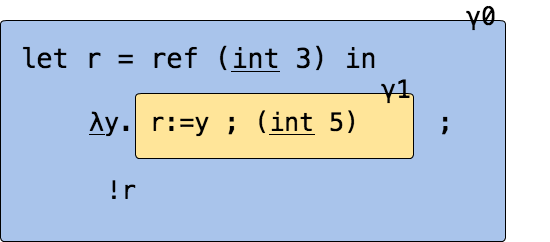
\includegraphics[clip,width=10cm]{./img/sudo_ref.png}
  \caption{危険な例}
  \label{fig:sudo_ref}
\end{figure}


ここで,$r$は,整数のコードを格納する参照(破壊的セル)であり,$r:=y$と
$!r$はそれぞれ,$r$への代入と$r$の中身の読み出しを表す.
上記のプログラムは,コードレベルのラムダ抽象($y$に対するラムダ抽象)で
生成されるコードレベル変数を$u$とするとき,$\code{u}$を$r$に格納し,
$u$のスコープ(黄色で示したもの)が終わったあとに取り出しているため,
計算結果は,自由変数をもつコード$\code{u}$となり,危険である.

上記のようなプログラムを型エラーとするため,須藤らは,コードレベル変数の
スコープごとに環境識別子を割り当てた.
上記では外側のスコープ(青)が$\gamma_0$,
内側のスコープ(黄)が$\gamma_1$という環境識別子で表現される.
$\gamma_0$で有効なコードレベル変数はなく,
$\gamma_1$で有効なコードレベル変数は$y$(に対応して生成される変数)である.
$\gamma_0$のスコープは$\gamma_1$のスコープを含む.言い換えれば,
$\gamma_1$で使える変数の方が$\gamma_0$で使える変数の方が(同じか)多い.
このことを$\gamma_1 \ord \gamma_0$ と表すことにする.
$r$は $\codeT{\intT}{\gamma_0} \mbox{\texttt{ref}}$型を持つ.
$y$は $\gamma_1$で使える変数であるが,$\gamma_0$では使えないため,
$r$に$y$を代入することはできず,$r:=y$のところで型エラーとなる.

コードレベルの変数スコープと,型によるスコープの表現をあらわしたのが,以下の図である.
forやletなどコードレベルの束縛子があるたびに,新しいスコープが開かれ,
使える変数が増えていくことが分かるだろう.

\begin{figure}[ht]
  \centering
  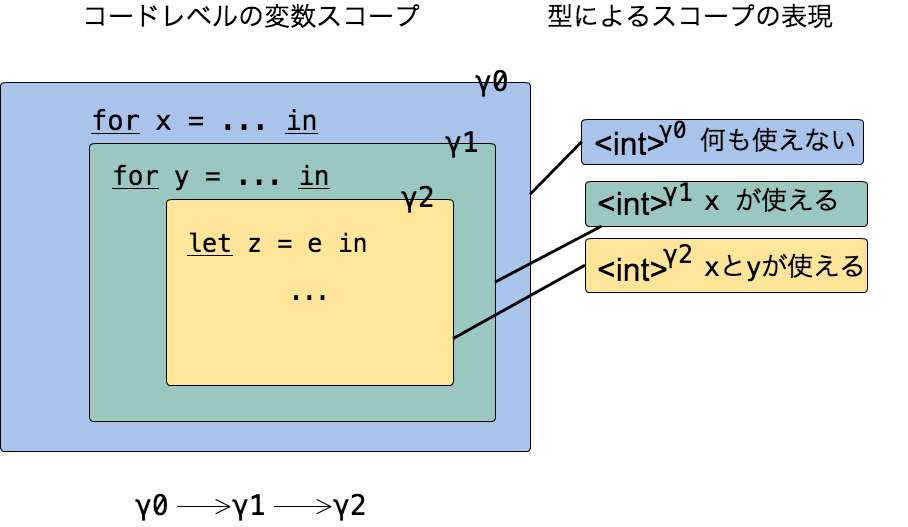
\includegraphics[clip,height=8cm]{./img/ec_for.png}
  \caption{型によるコードレベル変数のスコープ表現}
  \label{fig:ec_for}
\end{figure}

コードレベルの変数の型に,(精密化した)環境識別子を付与することで,その
変数が使えるスコープがわかり,破壊的代入などの副作用があるプログラムにおいても
スコープや型の安全性を保つことができる.

なお,須藤らの対象としていた言語が持っていた計算エフェクトは,「局所的なスコープをもつ参照」
であり,現実のOCaml/MetaOCaml等とは異なるものであった.
同一の著者グループは,最近,精密化した環境識別子のアイディアを用いて,
グローバルな参照を持つ言語に対するある種の型安全性
が成立することを示している\cite{Aplas2016}.

\section{本研究: 環境識別子の拡張}

本研究で扱う shift0/reset0によるコントロールエフェクトは,
須藤らによる精密化された環境識別子でも扱うことができない.本節では,そ
の問題点を明らかにし,その問題の解決の鍵となる join ($\cup$)の導入につ
いて述べる.

このため,前述の2重のforループ生成において,その中間にlet挿入をするプログラムに
ついて考察する.その概形は下記の1つ目の図である.

\begin{figure}[ht]
  \centering
  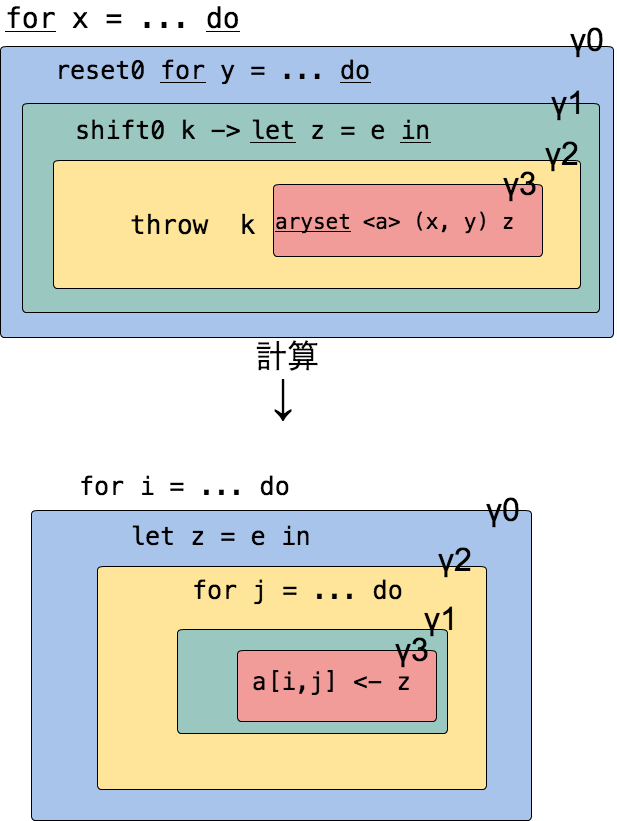
\includegraphics[clip,height=12cm]{./img/ecex_for_non_gamma.png}
  \caption{コード生成によるlet挿入}
  \label{fig:ecex_for_non_gamma}
\end{figure}

上の方の図で,使えるコードレベル変数が異なる場所ごとに,
$\gamma_0,\gamma_1,\gamma_2,\gamma_3$と名付けた.
須藤らの体系通りであれば,これらの環境識別子の間の順序は,スコープの包
含関係通りであるので,

\begin{figure}[ht]
  \centering
  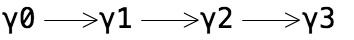
\includegraphics[clip,width=4cm]{./img/gamma_normal.png}
  \caption{誤った環境識別子の順序}
  \label{fig:gamma_normal}
\end{figure}

という順序がつくはずである.
しかし,計算を進めて得られたコードを見ると(上記の下の図はコードの中身を示している),
$\gamma_1$(緑色)と$\gamma_2$(黄色)の位置関係が入れ代わっている.
結果のコードの型が整合する(束縛変数が自由になることはない等)ために
は,$\gamma_2$において$\gamma_1$で使える変数を使ってはいけないことがわかる.
一方で,赤字で示された$\gamma_3$においては,$\gamma_1$の変数も
$\gamma_2$の変数も使って構わない.
これらを考慮すると,環境識別子の間の順序は以下の図となる.

\begin{figure}[ht]
  \centering
  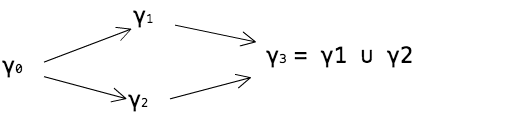
\includegraphics[clip,width=7cm]{./img/gamma.png}
  \caption{正しい環境識別子の順序}
  \label{fig:gamma}
\end{figure}

ここでのポイントは,$\gamma_0$ から,2つの異なる(包含関係のな
い)$\gamma_1$と$\gamma_2$に別れたあと,再び$\gamma_3$で合流することで
ある.須藤らの体系では,環境識別子のなす半順序集合全体は木の形であったが,
本研究の体系では,このように1度別れたものが合流することがある.
なお,$\gamma_3$で使える変数の集合は$\gamma_1$と$\gamma_2$で使える変数の和集
合と一致するので$\gamma_3 = \gamma_1 \cup \gamma_2$とおくことができる.
このように,環境識別子の世界に Join ($\cup$)を導入することによ
り,コントロールオペレータによる文脈の移動に対応できることになった.

\section{本研究: 型システムの構築}

本研究の基本アイディアは前項で述べたようなシンプルなものであるが,
言語体系と型システムの構築にあたってはいくつかの困難があった.
ここでは,そのうち,コントロールオペレータが切りとった継続に関する多相性について述べる.

前節の例では,shift0 が切り取る文脈(継続)は,
穴が$\gamma_1$のスコープにあり(その型は $\codeT{t_1}{\gamma_1}$の型),
文脈全体が$\gamma_0$のスコープのにある(その型は
$\codeT{t_0}{\gamma_0}$の形)となっている.
これをthrowにおいて使うときは,$\gamma_3$スコープのものを$\gamma_2$ス
コープに変換している.すなわち,$k$は $\codeT{t_1}{\gamma_3}$型
から$\codeT{t_0}{\gamma_2}$型への関数であるように振る舞う.

この2つのギャップを埋めるのは,継続(評価文脈)のある種の多相性である.
このケースでは,
\[\codeT{t_1}{\gamma_1} \to \codeT{t_0}{\gamma_0} \]
という型で定義された継続変数$k$が,任意の$\gamma_2 \ord \gamma_0$ に対して,
\[\codeT{t_1}{\gamma_1 \cup \gamma_2} \to \codeT{t_0}{\gamma_0 \cup \gamma_2} \]
という型を持つことが言えれば良いことがわかる.($\gamma_3 = \gamma_1
\cup \gamma_2$あること,また,$\gamma_2 \ord \gamma_0$ ならば
$\gamma_0 \cup \gamma_2 = \gamma_2$であることに注意されたい.)

このような多相性(サブタイプのもとでの多相性)は,継続の研究ではいくつか
知られており,今回のケースでも成立すると考えられる\footnote{この型付
  けが問題ないことは直感的には明らかであるが,
  意味論の上で,このような型付け規則が「正しい」ことの証明は,将来課題である.}.

本研究では,将来的に型推論アルゴリズムを構築することを考慮して,
環境識別子に関する一般的な多相性を導入することを避け,
継続変数について特別な型を与え,その変数をthrowで使うときに,
多相性を利用できるようにするという方策をとった.これにより型システムを
複雑化させることなく,コントロールオペレータの導入ができ,簡潔な型保存
性の証明につながった.

最終的に得られた throw の型付け規則は以下のものであり,
継続変数$k$ には,特別な関数型$\Rightarrow$を与えていること(通常の関数
型は$\rightarrow$で表現している),また,
$\gamma_1$から$\gamma_0$への変換子として得られた$k$を,
$\gamma_1\cup \gamma_2$から$\gamma_2 = \gamma_0 \cup \gamma_2$への
変換子として利用していることがわかる.
\[
  \infer
  {\Gamma,~k:\contT{\codeT{t_1}{\gamma_1}}{\codeT{t_0}{\gamma_0}}{\sigma}
    \vdash \throw{k}{v} : \codeT{t_0}{\gamma_2} ; \sigma}
  {\Gamma
    \vdash v : \codeT{t_1}{\gamma_1 \cup \gamma_2} ; \sigma
    & \Gamma \models \gamma_2 \ord \gamma_0
  }
\]

なお,継続が作用する型(上記の$\codeT{t_1}{\gamma_1}$など)は,本研究で
はコード型に限定した.その理由は,須藤らの体系の方式で,参照(ref)が関
数型を持つことを許すとコードレベル変数が束縛域を脱出してしまい,
本研究のコントロールオペレータを持つ体系でも同様の事態が生じると予想さ
れたからである.
なお,コード型のみを扱うことのできるコントロールオペレータであっても,
多段階let挿入の表現のためには十分である.

%%% Local Variables:
%%% mode: japanese-latex
%%% TeX-master: "master_oishi"
%%% End:

\chapter{対象言語: 構文と意味論}

本研究における対象言語は,ラムダ計算にコード生成機能とコントロールオペ
レータshift0/reset0を追加したものに型システムを導入したものである.

本稿では,最小限の言語のみについて考えるため,コード生成機能の
「ステージ(段階)」は,コード生成段階(レベル0,現在ステージ)と
生成されたコードの実行段階(レベル1,将来ステージ)の2ステージのみを考える.

前述したように,本研究の言語では,
コードコンビネータ(Code Combinator)方式を使い,
コードコンビネータは,
$\cPlus$ や $\cIf$のように下線を引いて表す.

\section{構文の定義}

対象言語の構文を定義する.

変数は,レベル0変数($x$), レベル1変数($u$),
(レベル0の)継続変数($k$)の3種類がある.
レベル0項($e^0$),レベル1項($e^1$)およびレベル0の値($v$)を下の通り定義する.

\begin{figure}[!ht]
  \centering
  \begin{align*}
    c & ::= i \mid b \mid \cint
        \mid \cat \mid + \mid \cPlus \mid \cIf \\
    v & ::= x \mid c \mid \fun{x}{e^0} \mid \code{e^1} \\
    e^0 & ::=  v  \mid e^0~ e^0 \mid \ift{e^0}{e^0}{e^0} \\
      & \mid \cfun{x}{e^0}
        \mid \ccfun{u}{e^0} \\
      & \mid \resetz{e^0}
        \mid \shiftz{k}{e^0}
        \mid \throw{k}{v} \\
    e^1 & ::=  u \mid c \mid \fun{u}{e^1} \mid e^1~ e^1
          \mid \ift{e^1}{e^1}{e^1} \\
  \end{align*}
  \caption{対象言語の構文の定義}
\end{figure}

ここで$i$は整数の定数,$b$は真理値定数である.

定数のうち,下線がついているものはコードコンビネータである.
変数は,ラムダ抽象(下線なし,下線つき,二重下線つき)および shift0 により束縛され,
$\alpha$同値な項は同一視する.
$\letin{x}{e_1}{e_2}$および$\clet{x}{e_1}{e_2}$は,
それぞれ,$(\fun{x}{e_2})e_1$ および $(\cfun{x}{e_2})\cat e_1$の省略形である.
前述の例でのべた$\cFor$は,
コード構築定数とコードレベル適用を用いて導入することとし,
(この導入にあたっての型システムの拡張は容易なので)ここでは省略する.

\section{操作的意味論}

対象言語は,値呼びで left-to-rightの操作的意味論を持つ.
ここでは評価文脈に基づく定義を与える.

評価文脈を以下のように定義する.
\begin{figure}[H]
  \centering
  \begin{align*}
    E & ::= [~] \mid E~ e^0 \mid v~ E \\
      & \mid \ift{E}{e^0}{e^0} \mid \Resetz~ E \mid \ccfun{u}{E}
  \end{align*}
  \caption{評価文脈}
\end{figure}

コード生成言語で特徴的なことは,
コードレベルのラムダ抽象の内部で評価が進行する点である.実際,
上記の定義には,$\ccfun{u}{E}$が含まれている.
たとえば,$\ccfun{u}{\code{u} \cPlus [~]}$ は評価文脈である.

この評価文脈$E$と次に述べる計算規則$r \to l$ により,
評価関係$e \lto e'$ を図\ref{fig:etoe}のように定義する.

\begin{figure}[H]
  \centering
  \[
    \infer{E[r] \lto E[l]}{r \to l}
  \]
  \caption{$e \lto e' $の評価関係}
  \label{fig:etoe}
\end{figure}


計算規則は図\ref{fig:calc_rule}の通り定義する.
\begin{figure}[H]
  \centering
  \begin{align*}
    (\fun{x}{e})~v &\to e\{ x := v \} \\
    \ift{true}{e_1}{e_2} &\to e_1 \\
    \ift{else}{e_1}{e_2} &\to e_2 \\
    \cfun{x}{e} &\to \ccfun{u}{(e\{ x := \code{u} \})} \\
    \ccfun{u}{\code{e}} &\to \code{\fun{u}{e}} \\
    \Resetz~ v &\to v \\
    \Resetz (E[\Shiftz~ k \to e]) &\to e \ksubst{k}{E}
  \end{align*}
  \caption{計算規則}
  \label{fig:calc_rule}
\end{figure}

ただし,4行目の$u$はフレッシュなコードレベル変数とし,
最後の行の$E$は穴の周りに{\Resetz}を含まない評価文脈とする.
また,この行の右辺のトップレベルに{\Resetz}がない点が,
shift/reset の振舞いとの違いである.すなわち,shift0 を1回計算すると,
reset0 が1つはずれるため,shift0 をN個入れ子にすることにより,
N個分外側のreset0 までアクセスすることができ,多段階let挿入を実現でき
るようになる.

上記における継続変数に対する代入$e\ksubst{k}{E}$は図\ref{fig:k_subst}の通り定義する.

\begin{figure}[H]
  \centering
  \begin{align*}
    (\throw{k}{v})\ksubst{k}{E} &\equiv \Resetz (E[v]) \\
    (\throw{k'}{v})\ksubst{k}{E} &\equiv \throw{k'}{(v\ksubst{k}{E})}
    \\
                                & \text{ただし}~k \not= k'
  \end{align*}
  \caption{継続への代入}
  \label{fig:k_subst}
\end{figure}

上記以外の$e$に対する代入の定義は透過的であるとする.
上記の定義の1行目で\Resetz を挿入しているのは{\Shiftz}の意味論に対応し
ており,これを挿入しない場合は別のコントロールオペレータ(Felleisenの
control/promptに類似した control0/prompt0)の振舞いとなる.

コードコンビネータ定数の振舞い(ラムダ計算における$\delta$規則に相当)は
図\ref{fig:comb-rule}のように定義する.

\begin{figure}[H]
  \centering
  \begin{align*}
    \cint~ n &\to \code{n} \\
    \code{e_1}~ \cat~ \code{e_2} &\to \code{e_1~ e_2} \\
    \code{e_1}~ \cPlus~ \code{e_2} &\to \code{e_1 + e_2} \\
    \cif{e_1}{e_2}{e_3} &\to \code{\ift{e_1}{e_2}{e_3}}
  \end{align*}
  \caption{コードコンビネータの規則}
  \label{fig:comb-rule}
\end{figure}

% 計算の例を以下に示す.
% \begin{align*}
    %     e_1 & = \Resetz ~~\cLet~x_1=\csp{3}~\cIn \\
    %               & \phantom{=}~~ \Resetz ~~\cLet~x_2=\csp{5}~\cIn \\
    %               & \phantom{=}~~ \Shiftz~k~\to~\cLet~y=t~\cIn \\
    %               & \phantom{=}~~ \Throw~ k~ (x_1~\cPlus~x_2~\cPlus~y) \\
    %   \end{align*}
    %
    %     \begin{align*}
    %     [ e_1 ] &\lto [ \Resetz (\cLet~x_1=\csp{3}~\cIn \\
    %               &\Resetz~ \cLet~x_2=\csp{5}~\cIn \\
    %               &[ \Shiftz~ k~ \to~ \cLet~ y=t~ \cIn \\
    %               &[ \Throw~ k~(x_1~\cPlus~x_2~\cPlus~y) ] ] ) ] \\
    %               &\lto [ \cLet~ y=t~ \cIn \\
    %               &[ \cfun{x}{\Resetz~ (\cLet~x_1=\csp{3}~ \cIn~ \Resetz~ (\cLet~ x_2=\csp{5}~ \cIn [x]))} (x_1~\cPlus~x_2~\cPlus~y) ]] \\
    %               &\lto [ \cfun{y}{(\cfun{x}{\Resetz~ (\cLet~x_1=\csp{3}~ \cIn~ \Resetz~ (\cLet~ x_2=\csp{5}~ \cIn [x]))} (x_1~\cPlus~x_2~\cPlus~y))}~ \cat~ t ] \\
    %               &\lto [[\cfun{y}{(\cfun{x}{\Resetz~ (\cLet~x_1=\csp{3}~ \cIn~ \Resetz~ (\cLet~ x_2=\csp{5}~ \cIn [x]))} (x_1~\cPlus~x_2~\cPlus~y))}]~ \cat~ t] \\
    %               &\lto [[\ccfun{y_1}{(\cfun{x}{\Resetz~ (\cLet~x_1=\csp{3}~ \cIn~ \Resetz~ (\cLet~ x_2=\csp{5}~ \cIn [x]))} (x_1~\cPlus~x_2~\cPlus~ \code{y_1}))}]~ \cat~ t] \\
    %               &\lto
                      %   \end{align*}

                      %%%   Local Variables:
                      %%%   mode: japanese-latex
                      %%%   TeX-master: "master_oishi"
                      %%%   End:

\chapter{型システム}

本研究での型システムについて述べる.

基本型$b$,環境識別子(Environment Classifier)$\gamma$を以下の通り定義する.

\begin{figure}[H]
  \centering
  \begin{align*}
    b & ::= \intT \mid \boolT \\
    \gamma & ::= \gamma_x \mid \gamma \cup \gamma
  \end{align*}
  \caption{基本型,環境識別子の定義}
  \label{fig:bec_def}
\end{figure}

$\gamma$の定義における$\gamma_x$は環境識別子の変数を表す.
すなわち,環境識別子は,変数であるかそれらを$\cup$で結合した形である.
以下では,メタ変数と変数を区別せず$\gamma_x$を$\gamma$と表記する.
ここで環境識別子として$\cup$を導入した理由は後述する.

$L ::= \empty \mid \gamma$ は現在ステージ(レベル0)と将来ステージ(レベル1)をまとめ
て表す記号である.たとえば,$\Gamma \vdash^L
e:t~;~\sigma$は,$L=\empty$のとき現在ステージ(レベル0)の判断で,
$L=\gamma$のとき将来ステージ(レベル1)の判断となる.

レベル0の型$t^0$,レベル1の型$t^1$,(レベル0の)型の有限列$\sigma$,
(レベル0の)継続の型$\kappa$を次の通り定義する.

\begin{figure}[H]
  \centering
  \begin{align*}
    t^0 & ::= b \mid \funT{t^0}{t^0}{\sigma} \mid \codeT{t^1}{\gamma} \\
    t^1 & ::= b \mid t^1 \to t^1 \\
    \sigma & ::= \epsilon \mid t^0, \sigma \\
    \kappa^0 & ::= \contT{\codeT{t^1}{\gamma}}{\codeT{t^1}{\gamma}}{\sigma}
  \end{align*}
  \caption{(レベル0の)継続の型の定義}
  \label{fig:k_def}
\end{figure}

レベル0の関数型$\funT{t^0}{t^0}{\sigma}$は,
エフェクトをあらわす列$\sigma$を伴っている.これは,その関数型をもつ項
を引数に適用したときに生じる計算エフェクトであり,具体的には,
\Shiftz の answer type の列である.前述したようにshift0 は多段
階の reset0 にアクセスできるため,$n$個先のreset0 の answer typeまで記
憶するため,このように型の列$\sigma$で表現している.
ただし,本研究の範囲では,answer type modification に対応する必要はな
いので,エフェクトはシンプルに型の列($n$個先の reset0 のanswer type を
$n=1,\cdots,k$に対して並べた列)で表現している.
この型システムの詳細は,Materzokら\cite{Materzok2011}の研究を参照されたい.

本稿の範囲では,コントロールオペレータは現在ステージ(レベル0)にのみあらわれ,生
成されるコードの中にはあらわないため,レベル1の関数型は,エフェクトを
表す列を持たない.
また,本項では,shift0/reset0 はコードを操作する目的にのみ使うため,継
続の型は,コードからコードへの関数の形をしている.
ここでは,後の定義を簡略化するため,継続を,通常の関数とは区別しており,
そのため,継続の型も通常の関数の型とは区別して二重の横線で表現している.

型判断は,以下の2つの形である.

\begin{figure}[H]
  \centering
  \begin{align*}
    \Gamma \vdash^{L} e : t ;~\sigma \\
    \Gamma \models \gamma \ord \gamma
  \end{align*}
  \caption{型判断の定義}
  \label{fig:judgement_def}
\end{figure}

ここで,型文脈$\Gamma$は次のように定義される.

\begin{figure}[H]
  \centering
  \begin{align*}
    \Gamma ::= \emptyset
    \mid \Gamma, (\gamma \ord \gamma)
    \mid \Gamma, (x : t)
    \mid \Gamma, (u : t)^{\gamma}
  \end{align*}
  \caption{型文脈の定義}
  \label{fig:type_context_def}
\end{figure}


型判断の導出規則を与える.まず,$\Gamma \models \gamma \ord \gamma$の
形に対する規則である.

\begin{figure}[H]
  \centering
  \[
    \infer
    {\Gamma \models \gamma_1 \ord \gamma_1}
    {}
    \quad
    \infer
    {\Gamma, \gamma_1 \ord \gamma_2 \models \gamma_1 \ord \gamma_2}
    {}
  \]

  \[
    \infer
    {\Gamma \models \gamma_1 \ord \gamma_3}
    {\Gamma \models \gamma_1 \ord \gamma_2 & \Gamma \models \gamma_2 \ord \gamma_3}
  \]

  \[
    \infer
    {\Gamma \models \gamma_1 \cup \gamma_2 \ord \gamma_1}
    {}
    \quad
    \infer
    {\Gamma \models \gamma_1 \cup \gamma_2 \ord \gamma_2}
    {}
  \]

  \[
    \infer
    {\Gamma \models \gamma_3 \ord \gamma_1 \cup \gamma_2}
    {\Gamma \models \gamma_3 \ord \gamma_1
      &\Gamma \models \gamma_3 \ord \gamma_2}
  \]
  \caption{$\Gamma \models \gamma \ord \gamma$の形に対する型導出規則}
  \label{fig:gmg_rule}
\end{figure}



次に,$\Gamma \vdash^{L} e : t ;~\sigma$ の形に対する型導出規則を与える.
まずは,レベル0における単純な規則である.

\begin{figure}[H]
  \centering
  \oishi{下の3つの型付け規則は$\Resetz$に対応する $\Shiftz, \Throw$がない場合でも,型が付いてほしいので,お尻に$\sigma$をつけている.つまり,$\Resetz~(\Resetz~ e)$ みたいなものでも型がつく.
  絶対に$\Resetz, \Shiftz, \Throw$の三位一体を条件として使うのならば,お尻に$\sigma$はいらないはず.($\Resetz$ で付加された answer type は $\Throw$のところで消えるから)}
  \[
    \infer
    {\Gamma, x : t \vdash x : t ~;~ \sigma}
    {}
    \quad
    \infer
    {\Gamma, (u : t)^\gamma \vdash^\gamma u : t ~;~ \sigma}
    {}
  \]

  \[
    \infer
    {\Gamma \vdash^{L} c : t^c ~;~\sigma}
    {}
  \]

  \[
    \infer
    {\Gamma \vdash^{\gamma} e_1~ e_2 : t_1 ; \sigma}
    {\Gamma \vdash^{\gamma} e_1 : \funT{t_2}{t_1}{\sigma};~ \sigma
      & \Gamma \vdash^{\gamma} e_2 : t_2  ; \sigma
    }
    \quad
    \infer
    {\Gamma \vdash e_1 \, e_2 : t;~\sigma}
    {\Gamma \vdash e_1 : t_2 \to t_1;~\sigma
      &\Gamma \vdash e_2 : t_2;~\sigma
    }
  \]

  \[
    \infer
    {\Gamma \vdash \fun{x}{e} : \funT{t_1}{t_2}{\sigma} ~;~\sigma'}
    {\Gamma,~x : t_1 \vdash e : t_2 ~;~ \sigma}
    \quad
    \infer
    {\Gamma \vdash^\gamma \fun{u}{e} : \funT{t_1}{t_2}{} ~;~ }
    {\Gamma,~(u : t_1)^\gamma \vdash^\gamma e : t_2 ~;~  }
  \]

  \[
    \infer
    {\Gamma \vdash^{L} \ift{e_1}{e_2}{e_3} : t ~;~ \sigma}
    {\Gamma \vdash^{L} e_1 : \boolT ;~ \sigma
      & \Gamma \vdash^{L} e_2 : t ; \sigma
      & \Gamma \vdash^{L} e_3 : t ; \sigma}
  \]
  \caption{(レベル0,レベル1の)$\Gamma \vdash^{L} e : t ;~\sigma$ の単純な形に対する型導出規則}
  \label{fig:gvs_rule}
\end{figure}


次にコードレベル変数に関するラムダ抽象の規則である.

\begin{figure}[H]
  \centering
  \[
    \infer[(\gamma_1~\text{is eigen var})]
    {\Gamma \vdash \cfun{x}{e} : \codeT{t_1\to t_2}{\gamma} ~;~ \sigma}
    {\Gamma,~\gamma_1 \ord \gamma,~x:\codeT{t_1}{\gamma_1} \vdash e
      : \codeT{t_2}{\gamma_1}; \sigma}
  \]
  \caption{コードレベルのラムダ抽象の型導出規則}
  \label{fig:code_abs_type_rule}
\end{figure}


コントロールオペレータに対する型導出規則である.

\begin{figure}[H]
  \centering
  \[
    \infer{\Gamma \vdash \resetz{e} : \codeT{t}{\gamma} ~;~ \sigma}
    {\Gamma \vdash e : \codeT{t}{\gamma} ~;~ \codeT{t}{\gamma}, \sigma}
  \]

  % \oishi{$\Throw$ルールの $\sigma$-part がずれる問題は $\Resetz$を $\Throw$の間に入れて対処していたが,$\Shiftz$で,$e$ の$\sigma$-part は先頭要素を減らさず,$\Throw$で減らすようにするのはどうか($\Resetz, \Shiftz, \Throw$は三位一体なので) → だめだった.shift をネストさせると,うまくいかないことがわかった}
  \[
    \infer{\Gamma \vdash \shiftz{k}{e} : \codeT{t_1}{\gamma_1} ~;~ \codeT{t_0}{\gamma_0},\sigma}
    {\Gamma,~k:\contT{\codeT{t_1}{\gamma_1}}{\codeT{t_0}{\gamma_0}}{\sigma}
      \vdash e : \codeT{t_0}{\gamma_0} ; \sigma
      & \Gamma \models \gamma_1 \ord \gamma_0
    }
  \]

  % \oishi{$\Shiftz$ルールでなく,$\Throw$ルールで対応するanswer type($\sigma$の先頭要素$\codeT{t'}{\gamma'}$)を減らす.→ だめだった.shift をネストさせると,うまくいかないことがわかった(多分減らさなくても型は付くと思うけど)}
  \oishi{複数の$\Throw$を使う場合,$\sigma$-partのsub sumptionを使えば良い}
  \[
    \infer
    {\Gamma,~ k:\contT{\codeT{t_1}{\gamma_1}}{\codeT{t_0}{\gamma_0}}{\sigma}
      \vdash \throw{k}{v} : \codeT{t_0}{\gamma_2} ; \sigma}
    {\Gamma,~ k:\contT{\codeT{t_1}{\gamma_1}}{\codeT{t_0}{\gamma_0}}{\sigma}
      \vdash v : \codeT{t_1}{\gamma_1 \cup \gamma_2} ; \sigma
      & \Gamma \models \gamma_2 \ord \gamma_0
    }
  \]
  \caption{コントロールオペレータに対する型導出規則}
  \label{fig:controlop_type_rule}
\end{figure}


コード生成に関する補助的な規則として,Subsumptionに相当する規則等がある.

% \oishi{$\ord$ の左右の $\gamma$ は逆? 一般に項の内部に入るにしたがって,使えるコードレベル変数は増えていくので,逆のような気がする.$ \gamma_1 \ord \gamma_0$ の意味は $\gamma_0$ より $\gamma_1$ のほうが使えるコードレベル変数は多いという意味である}

\begin{figure}[H]
  \centering
  \[
    \infer
    {\Gamma \vdash e : \codeT{t}{\gamma_2} ; \sigma}
    {\Gamma \vdash e : \codeT{t}{\gamma_1} ; \sigma
      & \Gamma \models \gamma_2 \ord \gamma_1
    }
  \]

  \[
    \infer
    {\Gamma \vdash^{\gamma_2} e : t ~;~ \sigma}
    {\Gamma \vdash^{\gamma_1} e : t ~;~ \sigma
      & \Gamma \models \gamma_2 \ord \gamma_1
    }
  \]


  \[
    \infer
    {\Gamma \vdash \code{e} : \codeT{t^1}{\gamma} ; \sigma}
    {\Gamma \vdash^{\gamma} e : t^1 ; \sigma}
  \]

  \[
    \infer
    {\Gamma \vdash e : t;~\codeT{t'}{\gamma_2},\sigma}
    {\Gamma \vdash e : t;~\codeT{t'}{\gamma_1},\sigma
      & \Gamma \models \gamma_2 \ord \gamma_1
    }
  \]

  \caption{コード生成に関するSubsumptionの型導出規則}
  \label{fig:code_gen_subs_type_rule}
\end{figure}

\Shiftz の Answer type の列($\sigma$)に関するSubsumptionに相当する規則がある.

\begin{figure}[H]
  \centering
  \[
    \infer
    {\Gamma \vdash e : t;~\codeT{t'}{\gamma_2},\sigma}
    {\Gamma \vdash e : t;~\codeT{t'}{\gamma_1},\sigma
      & \Gamma \models \gamma_2 \ord \gamma_1
    }
  \]
  \caption{$\sigma$-partに関するSubsumptionの型導出規則}
  \label{fig:sigma_subs_type_rule}
\end{figure}

\section{型付け例}

上記の型システムのもとで,いくつかの項の型付けについて述べる.

\subsection{let挿入の例}
\label{subsec:exam-let}


\begin{align*}
  e_1 & = \Resetz ~~\cLet~x_1= e_1 ~\cIn \\
      & \phantom{=}~~ \Resetz ~~\cLet~x_2= e_2~\cIn \\
      & \phantom{=}~~ \Shiftz~k~\to~\cLet~y=t~\cIn \\
      & \phantom{=}~~ \Throw~ k~ y
\end{align*}

式$e_1$に対して,$t=\cint~ 7$ あるいは $t=x_1$であれば,
$e_1$ は型付け可能である.
一方,$t=x_2$ であれば,$e_1$ は型付けできない.

\newcommand\tzero{\codeT{t}{\gamma_0}}
\newcommand\tone{\codeT{t}{\gamma_1}}
\newcommand\ttwo{\codeT{t}{\gamma_2}}
\newcommand\tthree{\codeT{t}{\gamma_3}}
\newcommand\tonethree{\codeT{t}{\gamma_1\uni\gamma_3}}
\newcommand\tall{\codeT{t}{\gamma_2\uni\gamma_1\uni\gamma_3}}
\newcommand\Gammaone{
  \longer{\gamma_1}{\gamma_0},~x_1:\tone \vdash
  \cLet~x_2=e_2~\cIn~\cdots : \tone;~\tone,\tzero}
\newcommand\Gammatwo{
  \Gamma_1,~k_2:\contT{\ttwo}{\tone}{\tzero},
  ~k_1:\contT{\tone}{\tzero}{\cdot{}}}

\def\proofone{
  \infer
  {\vdash e_1:\tzero;~\cdot{}}
  {
    \infer{\vdash \cLet~x_1=e_1~\cIn~\Resetz~\cLet~x_2=e_2~\cIn~\cdots :
      \tzero;~\tzero
    }
    {\infer{\longer{\gamma_1}{\gamma_0},~x_1:\tone \vdash
        \Resetz~\cLet~x_2=e_2~\cIn~\cdots : \tone;~\tzero
      }
      {\prooftwo}
    }
  }
}
\def\prooftwo{
  \infer{\longer{\gamma_1}{\gamma_0},~x_1:\tone \vdash
    \cLet~x_2=e_2~\cIn~\cdots : \tone;~\tone,\tzero}
  {\infer{\Gamma_1=\longer{\gamma_2}{\gamma_1},~x_2:\ttwo,~\longer{\gamma_1}{\gamma_0},~x_1:\tone \vdash
      \shiftz{k}{\cdots} : \ttwo;~\tone,\tzero
    }
    {\proofthree}
  }
}

\def\proofthree{
  {\infer{\Gamma_2=\Gamma_1,~k:\contT{\ttwo}{\tone}{\tzero}
      \vdash \cLet~y=t~\cIn~\cdots : \tone;~\tzero
    }
    {\prooffour}
  }
}

\def\prooffour{
  \infer{\Gamma_3=\Gamma_2,~\longer{\gamma_3}{\gamma_1},~y:\tthree \vdash \throw{k}{(\Resetz~ y)} :
    \tthree;~\tzero}
  {\infer{\Gamma_3 \vdash y : \tall;~\cdot}{\vdots}
    & \infer{\Gamma_3 \models \longer{\gamma_1\uni\gamma_3}{\gamma_1}}{}
  }
  & \infer[(*)]{\Gamma_2 \vdash t : \tone;~ \tzero}{\vdots}
}

\[
  \proofone
\]

$t$ が $x_1, \cint 7, x_2$ の場合に$\Gamma_2 \vdash t : \tone;~ \tzero$が成り立つかを見ていく.\\
$(*)$ のところに着目すると,
$\Gamma_2 = \longer{\gamma_2}{\gamma_1},~x_2:\ttwo,~\longer{\gamma_1}{\gamma_0},~x_1:\tone,~k:\contT{\ttwo}{\tone}{\tzero}$
より,
\begin{description}
\item[$t=x_1$の時]\mbox{}\\
  $x_1:\tone \vdash x_1:\tone$ が成り立ち,型が付く
\item[$t= \cint 7$の時]\mbox{}\\
  $\cint 7$ は定数であるので,どの Classifier $\gamma_i$ においても型が付く.
\item[$t=x_2$の時]\mbox{}\\
  $\longer{\gamma_2}{\gamma_1},~\longer{\gamma_1}{\gamma_0},~x_2:\ttwo$ より,
  $x_2$ のスコープは$\gamma_2$ であり,
  $\gamma_2$スコープのコード変数は,$\gamma_1$スコープでは一般に使用できないので
  $\longer{\gamma_2}{\gamma_1},~\longer{\gamma_1}{\gamma_0},~x_2:\ttwo \vdash x_2:\tone$ は成り立たず,型がつかない
\end{description}

\subsection{多段階let挿入の例}

\begin{align*}
  e_2 & = \Resetz ~~\cLet~x_1= e_1~\cIn \\
      & \phantom{=}~~ \Resetz ~~\cLet~x_2=e_2~\cIn \\
      & \phantom{=}~~ \Shiftz~k_2~\to~ \Shiftz~k_1~\to~ \cLet~y=t~\cIn \\
      & \phantom{=}~~ \Throw~k_1~ (\Resetz~ (\Throw~k_2~ y))
\end{align*}

式$e_2$に対して,$t=\cint7$であれば$e_1$は型付け可能である.
一方,$t=x_2$ あるいは $t=x_1$であれば,$e_1$は型付けできない.

\def\proofone{
  \infer
  {\vdash e:\tzero;~\cdot{}}
  {
    \infer{\vdash \cLet~x_1=e_1~\cIn~\Resetz~\cLet~x_2=e_2~\cIn~\cdots :
      \tzero;~\tzero
    }
    {\infer{\longer{\gamma_1}{\gamma_0},~x_1:\tone \vdash
        \Resetz~\cLet~x_2=e_2~\cIn~\cdots : \tone;~\tzero
      }
      {\prooftwo}
    }
  }
}
\def\prooftwo{
  \infer{\longer{\gamma_1}{\gamma_0},~x_1:\tone \vdash
    \cLet~x_2=e_2~\cIn~\cdots : \tone;~\tone,\tzero}
  {\infer{\Gamma_1=\longer{\gamma_2}{\gamma_1},~x_2:\ttwo,~\longer{\gamma_1}{\gamma_0},~x_1:\tone \vdash
      \shiftz{k_2}{\shiftz{k_1}{\cdots}} : \ttwo;~\tone,\tzero
    }
    {\proofthree}
  }
}

\def\proofthree{
  \infer{\Gamma_1,~k_2:\contT{\ttwo}{\tone}{\tzero}
    \vdash \shiftz{k_1}{\cdots} : \tone;~ \tzero
  }
  {\infer{\Gamma_2=\Gamma_1,~k_2:\contT{\ttwo}{\tone}{\tzero},
      ~k_1:\contT{\tone}{\tzero}{\cdot{}}
      \vdash \cLet~ y=t~ \cIn~\cdots : \tzero;~\cdot{}
    }
    {\prooffour}
  }
}

\def\prooffour{
  \infer{\Gamma_3=\Gamma_2,~\longer{\gamma_3}{\gamma_0},~y:\tthree \vdash \throw{k_1}{(\Resetz(\throw{k_2}{y}))} : \tthree;~\cdot{}}
  {\prooffive}
  & \infer[(*)]{\Gamma_2 \vdash t : \tzero;~ \cdot}{\vdots}
}

\def\prooffive{
  \infer
  {\Gamma_3 \vdash \Resetz(\throw{k_2}{y}) : \tonethree; ~\cdot{}}
  {\infer[(\#)]
    {\Gamma_3 \vdash \throw{k_2}{y} : \tonethree;~\tonethree}
    {\infer
      {\Gamma_3 \vdash \throw{k_2}{y} : \tonethree;~\tzero}
      {\Gamma_3 \vdash y :
        \codeT{t}{\gamma_2\uni\gamma_1\uni\gamma_3};~\cdot
        & \infer{\Gamma_3 \models
          \longer{\gamma_1\uni\gamma_3}{\gamma_0}}{}
      }
      & \infer{\Gamma_3 \models \longer{\gamma_1\uni\gamma_3}{\gamma_0}}{}
    }
  }
  & \infer{\Gamma_3 \models \longer{\gamma_3}{\gamma_0}}{}
}

\[
  \proofone
\]

この型付けで注意するところは,複数回の$\Throw$ を使うときは その間に $\Resetz$ を入れなければいけないところである.
$\Resetz$ を入れることで,$\sigma$-part のずれを防ぎ,$\Throw$ 規則を適用できる準備ができる.\\
$(\#)$のところに着目すると,$k_2$ の型は $k_2:\contT{\ttwo}{\tone}{\tzero}$ となっているので,$\Throw$規則を適用するには,$\sigma$-part の subsumption 規則を適用して $\tonethree$ から $\tzero$ が導ければ良い.

次に,$t$ が $x_1, x_2, \cint 7$ の場合に$\Gamma_2 \vdash t : \tzero;~ \cdot$が成り立つかを見ていく.\\
$(*)$ のところに着目すると,
$\Gamma_2 = \longer{\gamma_2}{\gamma_1},~x_2:\ttwo,~\longer{\gamma_1}{\gamma_0},~x_1:\tone,k_2:\contT{\ttwo}{\tone}{\tzero},~k_1:\contT{\tone}{\tzero}{\cdot{}}$
より,
\begin{description}
\item[$t=x_1$の時]\mbox{}\\
  $~\longer{\gamma_1}{\gamma_0},~x_1:\tone$ より,
  $x_1$ のスコープは$\gamma_1$ であり,
  $\gamma_1$スコープのコード変数は,$\gamma_0$スコープでは一般に使用できないので
  $~\longer{\gamma_1}{\gamma_0},~x_1:\tone \vdash x_2:\tzero$ は成り立たず,型がつかない
\item[$t=x_2$の時]\mbox{}\\
  $\longer{\gamma_2}{\gamma_1},~\longer{\gamma_1}{\gamma_0},~x_2:\ttwo$ より,
  $x_2$ のスコープは$\gamma_2$ であり,
  $\gamma_2$スコープのコード変数は,$\gamma_0$スコープでは一般に使用できないので
  $\longer{\gamma_2}{\gamma_1},~\longer{\gamma_1}{\gamma_0},~x_2:\ttwo \vdash x_2:\tzero$ は成り立たず,型がつかない
\item[$t= \cint 7$の時]\mbox{}\\
  $\cint 7$ は定数であるので,どの Classifier $\gamma_i$ においても型が付く.
\end{description}

このように,(少なくとも)上記の例については安全な式と危険な式(Scope extrusionが起こる式)を正しく選別できていることがわかった.

\section{型安全性について}

本研究の型システムに対する型保存(Subject Reduction)定理について述べる.
型保存定理は,(証明できれば)
進行(Progress)定理とあわせて型システムの健全性を導く定理である.

\begin{quote}
  (型保存性)
  $\vdash e:t~;~\sigma$ かつ $e \lto e'$ であれば,$\vdash e':t~;~\sigma$
  である.
\end{quote}

この定理は reset0-shift0の計算規則が多相性を持たない場合には容易に証明
できるが,多相性については精密な扱いが必要であり,
現段階では,型保存定理の証明は進行中である.


% \begin{lemm}[不要な仮定の除去]
%   $\Gamma_1,\gamma_2 \ord \gamma_1 \vdash e : t_1 ~;~\sigma$
%   かつ,$\gamma_2$が $\Gamma_1, e, t_1, \sigma$に出現しないなら,
%   $\Gamma_1 \vdash e : t_1 ~;~\sigma$ である.
% \end{lemm}
%
% \begin{lemm}[値に関する性質]
%   $\Gamma_1 \vdash v : t_1 ~;~\sigma$
%   ならば,
%   $\Gamma_1 \vdash v : t_1 ~;~\sigma'$
%   である.
% \end{lemm}
%
% \begin{lemm}[代入]
%   $\Gamma_1, \Gamma_2, x : t_1 \vdash e : t_2 ~;~\sigma$
%   かつ
%   $\Gamma_1 \vdash v : t_1 ~;~\sigma$
%   ならば,
%   $\Gamma_1, \Gamma_2 \vdash e\{x := v\} : t_2~;~\sigma$
% \end{lemm}
%
% これらをもとに型保存定理を証明する.
% 本研究の対象言語は,コントロールオペレータが操作する対象となる式の型を
% コード型に限定するなど,注意深く設計しているので,ほとんどのケースの証
% 明はスムーズであるが,reset0-shift0 に関する計算規則(shift0 が評価文脈
% を捕捉して継続変数$k$に渡す規則)とthrowに関する計算規則では,
% サブタイプ多相性に相当する性質を使っているので,以下の技術的な補題が必
% 要である.
%
% \begin{lemm}[識別子に関する多相性]
%   穴の周りにreset0を含まない評価文脈$E$,変数$x$,
%   そして$\Gamma = (u_1:t_1)^{\gamma_1}, \cdots, (u_n:t_n)^{\gamma_n}$
%   かつ$i=1,\cdots,n$に対して$\Gamma \models \gamma_0 \ord \gamma_i$であるとする.
%   このとき,
%   $\Gamma, x:\codeT{t_0}{\gamma'} \vdash E[x] : \codeT{t_1}{\gamma_0} ~;~\sigma$
%   であれば,フレッシュな$\gamma$に対して,
%   $\Gamma, x:\codeT{t_0}{\gamma'\cup \gamma} \vdash
%   E[x] : \codeT{t_1}{\gamma_0 \cup \gamma} ~;~\sigma$
%   である.
% \end{lemm}
%
% この補題は,評価文脈$E$に対して,穴の型が$\codeT{t_0}{\gamma'}$で
% 評価文脈全体の型が$\codeT{t_1}{\gamma_0}$であれば,
% それぞれの環境識別子に$\gamma_2$を加えて,
% $\codeT{t_0}{\gamma'\cup \gamma}$型から,
% $\codeT{t_1}{\gamma_0\cup \gamma}$型への評価文脈として使ってもよい,
% ということを主張している.ここで $\gamma \ord \gamma_0$ なので,
% $\gamma$と$\gamma_0 \cup \gamma$は$\ord$の意味で等しくなり,
% $\codeT{t_1}{\gamma_0\cup\gamma}$型を持つ項は,
% $\codeT{t_1}{\gamma}$型も持つことがわかる.
% この定理により,shift0が捕捉した継続を(環境識別子について)多相的に使う
% ことが可能となり,reset0-shift0 の計算規則が正当化される.
%
% 上記の補題を証明すれば,型保存定理の証明の残りのケースは比較的容易であ
% る.なお,この補題を使うケースにおいて,定理の言明にあらわれる項$e$が
% 閉じた項であること(環境識別子に関する
%
%
% 進行定理については
% 精密な定式化が必要(reset0がない式でshift0を実行した時など)が必要なので,

% \section{進行}
% \begin{theo}[進行]
%   $\vdash e:t$ が導出可能であれば,$e$ は 値 $v$ である.または,$e \lto e'$ であるような 項 $e'$ が存在する
% \end{theo}
%
% \paragraph{証明}
% $\vdash e:t$ の導出に関する帰納法による.\\
% Const, Abs, Code 規則の場合 $e$ は値である.\\
% Var 規則の場合 $\vdash e:t$ は導出可能でない.\\
% Throw 規則の場合 $\vdash e:t$ は導出可能でない.\\
% Reset0 規則の場合 $e = \Resetz~ e_1$ とする.
% 帰納法の仮定より評価文脈における $\Resetz E$ より簡約が進み,\\
% $e_1$ が値のとき,$e \lto v$ となるような $v$ が存在する.\\
% $e_1$ が値でないとき,

%%% Local Variables:
%%% mode: japanese-latex
%%% TeX-master: "master_oishi"
%%% End:

\chapter{型推論}

概要: 以下の2ステップから構成
\begin{itemize}
\item 制約生成:与えられた項にたいして、(型およびクラシファイアに関する)制約を返す。
\item 制約を解く。
\end{itemize}

\section{制約生成}

これは、もの型システム($T_1$とする)を
「トップダウンでの制約生成向け型システム($T_2$とする)」に変
形することであたえる。

$T_2$の設計指針:
\begin{itemize}
\item $T_1$と$T_2$は「型付けできる」という関係として等価である。
\item $T_2$は、term-oriented である。
  (結論側の式のトップレベルの形だけで、どの型付けルールを適用可能か、一意的にわかる。)
\item $T_2$は、制約生成をする。
  (結論側の式の要素は変数として、
  「それがこういう形でなければいけない」という条件は、制約の形で「生成」する。)
\end{itemize}

以上をどう満たすか? ポイントは、subsumption rule の適用タイミング(な
るべく subsumption rule を適用するのを避けたい)である。

\section{型システム$T_2$の導入}

subsumption rule が出現する場所を限定することができる.
特に,ルールと,その直後に subsumption がつかわれる場合を考えてみよう.
以下で,「var1」等といった表記は,
「もともとあるver1ルールを subsumption規則と組み合わせた形に改訂したも
の」である.
また,横棒の右に書いてあるConstr;... は(ルールを下から上にむけて
使うとき),Constr 以下の制約が生成される,という意味である.

また、型$t_1, t_2$に対する$\longer{}{}$の記号は以下の意味であるが、
とりあえず、(以下の意味にしたがって分解はせずに)
$\longer{t_1}{t_2}$ の形のまま、制約として生成する。
\begin{itemize}
\item $\longer{\codeT{t_1}{\gamma_1}}{\codeT{t_2}{\gamma_2}}$
  は、「$t_1=t_2$ かつ $\longer{\gamma_1}{\gamma_2}$
\item $\codeT{t}{\gamma}$の形でない$t_1,t_2$に対しては、
  $t_1 = t_2$。
\end{itemize}
(型推論のプロセスの最中では、$t_1, t_2$ はメタ型変瑞。洽筅キ、譴此その場合、どちらの形かは決定できないので、$\longer{t_1}{t_2}$を
上記の意味にしたがって、「ほどく」ことはできない。なので、
$\longer{t_1}{t_2}$という形のまま制約として生成する。)

(亀山メモ:
ただ、もしかすると、
「レベル0の型変数」と「レベル1の型変数」を最初からわけておく方法もある
かもしれない。そうすると、上記はとける?)


\oishi{
  以下のルールにおいて,Constraint の $\Gamma \models \longer{t}{t'}$ の $\Gamma \models$ はルールを適用した瞬間の $\Gamma$ の情報は制約解消において使わないから必要ない?\\
  一貫性をもたせるのなら, $t = t'$ の形の Constraint も $\Gamma \models t = t'$ とする必要がある?
}
\\
(var0)

\[
  \infer[Constr;~\Gamma \models \longer{t}{t'}]
  {\Gamma \vdash x:t;~\sigma}
  {(x:t') \in \Gamma
  }
\]

(var1)

\[
  \infer[Constr;~\Gamma \models \longer{\gamma}{\gamma'}]
  {\Gamma \vdash^{\gamma} u:t;~\sigma}
  {(u:t)^{\gamma'} \in \Gamma
  }
\]

(const)

\[
  \infer[Constr;~\Gamma \models \longer{t}{t^c}]
  {\Gamma \vdash^{L} c:t;~\sigma}
  {}
\]

(app0)

\[
  \infer[Constr;~\Gamma \models \longer{t}{t_1}]
  {\Gamma \vdash^\gamma e_1 \, e_2 : t;~\sigma}
  {\Gamma \vdash^\gamma e_1 : \funT{t_2}{t_1}{\sigma};~\sigma
    &\Gamma \vdash^\gamma e_2 : t_2;~\sigma
  }
\]

(app1)

\[
  \infer[Constr;~\Gamma \models \longer{t}{t_1}]
  {\Gamma \vdash e_1 \, e_2 : t;~\sigma}
  {\Gamma \vdash e_1 : t_2 \to t_1;~\sigma
    &\Gamma \vdash e_2 : t_2;~\sigma
  }
\]

(lambda0)

\[
  \infer[Constr;~t=\funT{t_1}{t_2}{\sigma'},~ \Gamma \models \sigma \ord \sigma' ]
  {\Gamma \vdash \lambda x.e : t;~\sigma}
  {\Gamma,~x:t_1 \vdash e : t_2;~\sigma'}
\]

(lambda1) \\
\oishi{
  コードの中で,shift0/reset0 は使わないので, $\sigma$ は $\epsilon$ なはず.
  なので,$\sigma$ は $\epsilon$ としておいてもよい
}

\[
  \infer[Constr;~t=\funT{t_1}{t_2}{}]
  {\Gamma \vdash^\gamma \lambda u.e : t;~\sigma}
  {\Gamma,~(u:t_1)^\gamma \vdash^\gamma e : t_2;~\sigma}
\]

(if)

\[
  \infer[Constr;~(none)]
  {\Gamma \vdash^L
    \textbf{if}~e_1 \textbf{then}~e_2 \textbf{else}~e_3 ~:~t; ~ \sigma}
  {\Gamma \vdash^L e_1 : \Bool;~\sigma
    &\Gamma \vdash^L e_2 : t;~\sigma
    &\Gamma \vdash^L e_3 : t;~\sigma
  }
\]

(code-lambda)

\[
  \infer[Constr;~\Gamma \models \longer{t}{\codeT{t_1 \to t_2}{\gamma}}]
  {\Gamma \vdash \underline{\lambda}x.e ~:~t;~\sigma}
  {\Gamma,\longer{\gamma'}{\gamma},x:\codeT{t_1}{\gamma'}
    \vdash e : \codeT{t_2}{\gamma'};~\sigma
  }
\]

(reset0)

\[
  \infer[Constr;~\Gamma \models \longer{t}{\codeT{t'}{\gamma}}]
  {\Gamma \vdash \Resetz~e ~:~ t; ~\sigma}
  {\Gamma \vdash e:\codeT{t'}{\gamma};~\codeT{t'}{\gamma},\sigma
  }
\]

(shift0)

\[
  \infer[Constr;~\Gamma \models \longer{t}{\codeT{t_1}{\gamma_1}},~ t_2 =\codeT{t_0}{\gamma_0},~ \Gamma \models \longer{\gamma_1}{\gamma_0}]
  {\Gamma \vdash \shiftz{k}{e} : t~;~ t_2,\sigma}
  {\Gamma,~k:\contT{\codeT{t_1}{\gamma_1}}{\codeT{t_0}{\gamma_0}}{\sigma}
    \vdash e : \codeT{t_0}{\gamma_0} ; \sigma
  }
\]


(throw0)\\
\oishi{
  throw0 ルールにのみ $\sigma$ part の subsumption ルールを適用すればおk?
}
\\
変更前
\[
  \infer[Constr;~ \Gamma \models \longer{t}{\codeT{t_0}{\gamma_2}},~ (\Gamma,~ k:t') \models \gamma_2 \ord \gamma_0,~  t' = \contT{\codeT{t_1}{\gamma_1}}{\codeT{t_0}{\gamma_0}}{\sigma}]
  {\Gamma,~ k:t'
    \vdash \throw{k}{v} : t ; \sigma}
  {\Gamma,~ k:t'
    \vdash v : \codeT{t_1}{\gamma_1 \uni \gamma_2} ; \sigma
  }
\]

変更後
\[
  \infer[Constr;~ \Gamma \models \longer{t}{\codeT{t_0}{\gamma_2}},~ (\Gamma,~ k:t') \models \gamma_2 \ord \gamma_0,~  t' = \contT{\codeT{t_1}{\gamma_1}}{\codeT{t_0}{\gamma_0}}{\sigma},~ \Gamma \models \gamma_1 \uni \gamma_2 \ord \gamma']
  {\Gamma,~ k:t'
    \vdash \throw{k}{v} : t ; \sigma}
  {\Gamma,~ k:t'
    \vdash v : \codeT{t_1}{\gamma'} ; \sigma
  }
\]

(code)

\[
  \infer[Constr;~\longer{t}{\codeT{t_1}{\gamma}}]
  {\Gamma \vdash \code{e} : t;~\sigma}
  {\Gamma \vdash^\gamma e : t_1;~\sigma}
\]


この新しい型システム$T_2$ は(hopefully) $T_1$と同じ型付けをあたえる。

型推論では、与えられた項$e$に対して、
$T_2$を「下から上」の向きに適用して、Constraintを生成する。
(もちろん、途中で、つまってしまったら、型推論は失敗する。

下から上に行くときに、「横棒の下には存在しないで、横棒の上、あるいは、
Constraintの中にのみ存在する」型やclassifier があるときは、
これらを型変数やclassifier変数として生成する。

なお、code-lambda規則での新しいclassifier は、classfier変数ではなく、
classifier定数とする。(この段階では、変数も定数も差はないが、
制約を解消するとき、cassifier定数に対する代入はしない、という違いがある。)

\chapter{制約の解消}

制約生成が成功したとき(つまり、途中で「つっかかったり」しないとき)、以
下の性質が成立するはずである。

入力を$\Gamma, L, e, t,\sigma$ として、前章の制約生成アルゴリズムを走
らせ、それが成功して$C$という制約を生成したとき、
\begin{itemize}
\item
  $\Gamma \vdash^L e: t; ~ \sigma$ が導出可能ならば、
  $C$ を満たす解が存在し、
\item
  $C$ を満たす解が存在すれば、ある代入$\theta$に対して、
  $\Gamma\theta \vdash^L e\theta: t\theta; ~ \sigma\theta$ が導出可能である。
\end{itemize}
という性質が成立することができる。
(これが成立すれば、もともとの型推論問題を、型制約の解消問題に帰着できたことになる。)

というわけで、制約の解消をはじめよう。制約は以下の文法で与えられたものの有限集合である。

\begin{itemize}
\item $\Gamma \models \longer{t^0}{t^0}$
\item $\Gamma \models \longer{c}{c}$
\item $\Gamma \models \longer{\sigma}{\sigma}$
\item $t^0=t^0$
\item $t^1=t^1$
\end{itemize}
ただし、ここで $t_0$, $t_1$, $c$, $\sigma$ は以下の文法で定義される。

\begin{align*}
  t^0      & ::= t^0_x \mid \Int \mid \Bool \mid \funT{t^0}{t^0}{c} \mid \codeT{t^1}{c} \\
  t^1      & ::= t^1_x \mid \Int \mid \Bool \mid \funT{t^1}{t^1}{} \\
  c        & ::= \gamma \mid d \mid c \uni c \\
  \sigma   & ::= \epsilon \mid t^0, \sigma
\end{align*}


$t_0$, $t_1$, $c$, $\sigma$ はそれぞれ、
レベル0型、
レベル1型、
レベル0型の列,
classifierをあらわす表現(メタ変数),
である。また、
$t^i_x$はそれぞれのレベルの型変数、$\gamma$はclassifier変数である。
また、$d$は、固有変数条件をもつclassifier変数のことであり、
型推論のあいだは、これは(実質的に)定数として扱われる(つまり、
$d$に対しては代入しない。classifier変数$\gamma$に対しては代入する。)

また、$\Gamma$は、一般の型文脈であるが、不要な情報を落として以下の形にしてよい。
\begin{align*}
  \Delta & ::= \cdots \mid \Delta,\longer{d}{c}
\end{align*}
(左辺は、固有変数なので、classifier定数である。右辺は一般のclassifier
式がなんでも来る可能性がある。)

制約の解消とは、制約(上記の形の有限集合)が与えられたとき、
それの「解」となる代入をともとめることである。代入$S$は、
型変数$\alpha^0, \alpha^1$への型の代入と、
classifier変数$\gamma$へのclassifierの代入とから構成される。
この代入は「最も一般的」であるべきである。(定義の詳細はいまは省略)

\section{制約の解消アルゴリズム(前半)}

$t^0=s^0$ と $t^1=s^1$ の形の制約は、普通の型推論で解ける。
それを解いた結果、$\alpha^0$、$\alpha^1$, $\gamma$に対する代入が生じ
る(か、あるいは、「解なし」という結果になる)。

$\Delta \models \longer{t^0}{s^0}$の形の制約は、両方ともが型変数の場合以外は、
簡単に解ける。(その結果として、$t^i=s^i$ の型の制約や、$\Delta \models
\longer{c}{c}$の形の制約を生む可能性があるが、前者は前と同様に解けばよ
く、前者を解いている間にあらたに$\Delta \models \longer{t^0}{s^0}$の形の制約は生じない。)

ここまでの段階で(代入がいくつか出たほか)、残る制約は、以下のものだけである。

\begin{itemize}
\item $\Delta \models \longer{\alpha^0}{\beta^0}$
\item $\Delta \models \longer{c}{c}$
\end{itemize}

ここまでにでてきた代入はすべて、上記の制約たちに適用済みとする。」
(つまり、$\alpha:=\Int$という代入がでてきたら、上の式にある$\alpha$は
すべて$\Int$にしておく。その結果、「代入における左辺にでてくる型変数やclassifier変数」
は、上記の制約たちには、のこっていない。)


\section{制約の解消アルゴリズム(後半)}

$\Delta \models \longer{c}{c}$の形の制約を解こう。
($\Delta \models \longer{\alpha^0}{\beta^0}$については次のsectionで
考えるので、ここでは無私する。)

この形の制約たちを、
$\Delta_i \models \longer{c_i}{c'_i}$とすると、
それぞれの $\Delta_i$ はcompatible であるはずなので(ここはあとでチェッ
クが必要)
$\Delta = \Delta_1 \cup \cdots \cup \Delta_n$ という風に全部を合体させ
た上で、$\Delta \models \longer{c_i}{c'_i}$を解けばよい。

(ステップ1: classifier変数の除去)
使われているclassifier変数の1つに着目する。(どれでもよい。)それを
$\gamma$とする。
$\longer{c_i}{\gamma}$ の形の制約 ($i=1,2,\cdots,I$)とを全部あつめる。
$\longer{\gamma}{c'_j}$ の形の制約 ($j=1,2,\cdots,J$)と、
これらを消去して、かわりに、以下の制約を、すべての$(i,j)$に対して追加する。

\[
  \longer{c_i}{c'_j}
\]

これにより、classifier変数は1つ減る。(制約は一般には増えるかもしれない。)
ステップ1を繰返すと、classifier変数はなくなる。

(ステップ2) $\longer{c_1 \uni c_2}{c_3}$ を
$\longer{c_1}{c_3}$ と
$\longer{c_2}{c_3}$ に変換する。

これにより、不等号の左辺にある$\uni$の個数が1つ減る。
ステップ2を繰返すと、不等号の左辺にある$\uni$はなくなる。

ステップ2の繰返しがおわると、制約は、
$\Delta \models \longer{d}{c}$の形になる。

\oishi{ステップ3 は変更する必要あり }\\
(ステップ3) ここで「$d$は atomic」 という仮定をおく。これについては
あとで吟味する.
これは、
「$\longer{d}{c_1 \uni c_2}$ ならば
$\longer{d}{c_1}$または、
$\longer{d}{c_2}$」という内容である。
これらの逆向きは、いつでも成立するので、結局、ここの「ならば」は「同値」といってもよい。

これをもちいて、$\longer{d}{c}$の右辺も分解できて、

\[
  \Delta \models \longer{d_1}{d_1'} \vee \cdots \vee \longer{d_n}{d'_n}
\]

となり、さらに$\Delta$も $\longer{d1}{d2}$の形を「かつ」と「または」で
つないだ形になるはずである。

これは decidable なので、「解があるかどうか」もdecidableである。

\section{制約の解消アルゴリズム(後半のおまけ)}

実は、まだ、
$\Delta \models \longer{\alpha^0}{\beta^0}$という制約がのこっていた。

これを最後まで残した(解かなかった)のは、以下の2つの可能性があるからで
ある。これはどうするか?

\begin{itemize}
\item $\alpha^0 = \beta^0$
\item
  $\alpha^0 = \codeT{t}{\gamma1}$,
  $\beta^0 = \codeT{t}{\gamma2}$,
  $\Delta \models \longer{\gamma1}{\gamma2}$
\end{itemize}


%%% Local Variables:
%%% mode: japanese-latex
%%% TeX-master: "master_oishi"
%%% End:

\chapter{実装}
この章では,コード生成言語にshift0/reset0 を導入した言語の評価器と
その言語で記述した項に対して,型推論を行い,自動的に型を付けるために必要な制約を生成する制約生成器の実装を見ていく.なお,実際のプログラムソースは付録に掲載している.
それらの実装は OCaml を用いて実装を行っている.

\section{評価器}
\begin{itemize}
\item 評価器 \lstinline|eval1|は,項$e$を受け取り,値$v$を返す関数である.
\item プリティプリンタ \lstinline|print_expr'| は,項$e$ を受け取り,項$e$のASTを整形する関数である.
\item プリティプリンタ \lstinline|print_value'| は,値$v$ を受け取り,値$v$のASTを整形する関数である.
\end{itemize}

以下で,いくつか具体例を見ていく

\begin{lstlisting}
 let e1 =
  R0
   (PrimOp2 ("Add_", Code (Int 10),
     R0
      (PrimOp2 ("Add_", Code (Int 20),
        S0 ("k1",
         S0 ("k2",
          App (Var "k1", App (Var "k2", Code (Int 1)))))))));;

# print_expr' e1
R0(<10> +_ R0(<20> +_ (S0 k1 -> (S0 k2 -> (k1 (k2 <1>))))))- : unit = ()

#  print_value' (eval1 e1)
<20 + 10 + 1>- : unit = ()

\end{lstlisting}

\section{制約生成器}
制約生成器は, $T_2$の型付け規則を用い,下から上に型付けを行い制約を生成していく.
それによって,型とclassifierと$\sigma$-partに関する制約が生成され,
対応する型付け規則がなければ,そこで止まる.
\begin{itemize}
\item 制約生成器 \lstinline|pp_cnstrl|は,項$e$を受け取り,制約を整形した結果を返す関数である.
% \item プリティプリンタ \lstinline|print_cnstr'| は,制約を受け取り,そのASTを整形する関数である.
\end{itemize}

\ref{subsec:exam-let} のlet挿入の例に対して,どのような制約が現れるか以下に実行例を記す.

\tiny
\begin{lstlisting}
# pp_cnstrl (R0(Let_("x", Code(Int 1), R0(Let_("y", Code(Int 2), S0("k", Let_("z", Var "x", T0("k", App(Var "k", Var "z")))))))));;
t_161 = Int,
 |= <t_150>^(γ_159) > <t_161>^(γ_173),
 |= <t_149>^(γ_158) > <t_150>^(γ_159),
 |= t_148 > <t_149>^(γ_158),
t_160 = Int,
γ_160>γ_159,x: (<t_150>^(γ_160))^(lv0), |= <t_152>^(γ_162) >
 <t_160>^(γ_172),
γ_160>γ_159,x: (<t_150>^(γ_160))^(lv0), |= <t_151>^(γ_161) >
 <t_152>^(γ_162),
γ_160>γ_159,x: (<t_150>^(γ_160))^(lv0), |= <t_150>^(γ_160) >
 <t_151>^(γ_161),
 |= <t_149>^(γ_158) > <t_150>^(γ_159),
 |= t_148 > <t_149>^(γ_158),
k: (<t_154>^(γ_165) = <t_149>^(γ_158),ε  => <t_153>^(γ_164))^(lv0),
γ_163>γ_162,
y: (<t_152>^(γ_163))^(lv0),γ_160>γ_159,x: (<t_150>^(γ_160))^(lv0), |=
 <t_155>^(γ_166) > <t_150>^(γ_160),
k: (<t_154>^(γ_165) = <t_149>^(γ_158),ε  => <t_153>^(γ_164))^(lv0),
γ_163>γ_162,
y: (<t_152>^(γ_163))^(lv0),γ_160>γ_159,x: (<t_150>^(γ_160))^(lv0), |=
 <t_153>^(γ_164) > <t_155>^(γ_166),
γ_163>γ_162,
y: (<t_152>^(γ_163))^(lv0),γ_160>γ_159,x: (<t_150>^(γ_160))^(lv0), |=
 <t_152>^(γ_163) > <t_154>^(γ_165),
<t_151>^(γ_161) = <t_153>^(γ_164),
γ_163>γ_162,
y: (<t_152>^(γ_163))^(lv0),γ_160>γ_159,x: (<t_150>^(γ_160))^(lv0), |=
 γ_165 > γ_164,
γ_160>γ_159,x: (<t_150>^(γ_160))^(lv0), |= <t_151>^(γ_161) >
 <t_152>^(γ_162),
γ_160>γ_159,x: (<t_150>^(γ_160))^(lv0), |= <t_150>^(γ_160) >
 <t_151>^(γ_161),
 |= <t_149>^(γ_158) > <t_150>^(γ_159),
 |= t_148 > <t_149>^(γ_158),
γ_167>γ_166,
z: (<t_155>^(γ_167))^(lv0),
k: (<t_154>^(γ_165) = <t_149>^(γ_158),ε  => <t_153>^(γ_164))^(lv0),
γ_163>γ_162,
y: (<t_152>^(γ_163))^(lv0),γ_160>γ_159,x: (<t_150>^(γ_160))^(lv0), |=
 t_159 -> t_158 > <t_154>^(γ_165) = <t_149>^(γ_158),ε  => <t_153>^(γ_164),
γ_167>γ_166,
z: (<t_155>^(γ_167))^(lv0),
k: (<t_154>^(γ_165) = <t_149>^(γ_158),ε  => <t_153>^(γ_164))^(lv0),
γ_163>γ_162,
y: (<t_152>^(γ_163))^(lv0),γ_160>γ_159,x: (<t_150>^(γ_160))^(lv0), |=
 <t_157>^(γ_171) > t_158,
γ_167>γ_166,
z: (<t_155>^(γ_167))^(lv0),
k: (<t_154>^(γ_165) = <t_149>^(γ_158),ε  => <t_153>^(γ_164))^(lv0),
γ_163>γ_162,
y: (<t_152>^(γ_163))^(lv0),γ_160>γ_159,x: (<t_150>^(γ_160))^(lv0), |=
 <t_155>^(γ_167) > <t_156>^(γ_170),
γ_167>γ_166,
z: (<t_155>^(γ_167))^(lv0),
k: (<t_154>^(γ_165) = <t_149>^(γ_158),ε  => <t_153>^(γ_164))^(lv0),
γ_163>γ_162,
y: (<t_152>^(γ_163))^(lv0),γ_160>γ_159,x: (<t_150>^(γ_160))^(lv0), |=
 γ_170 > γ_168,
<t_154>^(γ_165) = <t_149>^(γ_158),ε  => <t_153>^(γ_164) =
 <t_157>^(γ_169) = <t_151>^(γ_161),<t_149>^(γ_158),ε   => <t_156>^(γ_168),
γ_167>γ_166,
z: (<t_155>^(γ_167))^(lv0),
k: (<t_154>^(γ_165) = <t_149>^(γ_158),ε  => <t_153>^(γ_164))^(lv0),
γ_163>γ_162,
y: (<t_152>^(γ_163))^(lv0),γ_160>γ_159,x: (<t_150>^(γ_160))^(lv0), |=
 γ_169 U γ_170 > γ_171,
k: (<t_154>^(γ_165) = <t_149>^(γ_158),ε  => <t_153>^(γ_164))^(lv0),
γ_163>γ_162,
y: (<t_152>^(γ_163))^(lv0),γ_160>γ_159,x: (<t_150>^(γ_160))^(lv0), |=
 <t_153>^(γ_164) > <t_155>^(γ_166),
γ_163>γ_162,
y: (<t_152>^(γ_163))^(lv0),γ_160>γ_159,x: (<t_150>^(γ_160))^(lv0), |=
 <t_152>^(γ_163) > <t_154>^(γ_165),
<t_151>^(γ_161) = <t_153>^(γ_164),
γ_163>γ_162,
y: (<t_152>^(γ_163))^(lv0),γ_160>γ_159,x: (<t_150>^(γ_160))^(lv0), |=
 γ_165 > γ_164,
γ_160>γ_159,x: (<t_150>^(γ_160))^(lv0), |= <t_151>^(γ_161) >
 <t_152>^(γ_162),
γ_160>γ_159,x: (<t_150>^(γ_160))^(lv0), |= <t_150>^(γ_160) >
 <t_151>^(γ_161),
 |= <t_149>^(γ_158) > <t_150>^(γ_159),
 |= t_148 > <t_149>^(γ_158),
γ_167>γ_166,
z: (<t_155>^(γ_167))^(lv0),
k: (<t_154>^(γ_165) = <t_149>^(γ_158),ε  => <t_153>^(γ_164))^(lv0),
γ_163>γ_162,
y: (<t_152>^(γ_163))^(lv0),γ_160>γ_159,x: (<t_150>^(γ_160))^(lv0), |=
 t_159 > <t_155>^(γ_167),
γ_167>γ_166,
z: (<t_155>^(γ_167))^(lv0),
k: (<t_154>^(γ_165) = <t_149>^(γ_158),ε  => <t_153>^(γ_164))^(lv0),
γ_163>γ_162,
y: (<t_152>^(γ_163))^(lv0),γ_160>γ_159,x: (<t_150>^(γ_160))^(lv0), |=
 <t_157>^(γ_171) > t_158,
γ_167>γ_166,
z: (<t_155>^(γ_167))^(lv0),
k: (<t_154>^(γ_165) = <t_149>^(γ_158),ε  => <t_153>^(γ_164))^(lv0),
γ_163>γ_162,
y: (<t_152>^(γ_163))^(lv0),γ_160>γ_159,x: (<t_150>^(γ_160))^(lv0), |=
 <t_155>^(γ_167) > <t_156>^(γ_170),
γ_167>γ_166,
z: (<t_155>^(γ_167))^(lv0),
k: (<t_154>^(γ_165) = <t_149>^(γ_158),ε  => <t_153>^(γ_164))^(lv0),
γ_163>γ_162,
y: (<t_152>^(γ_163))^(lv0),γ_160>γ_159,x: (<t_150>^(γ_160))^(lv0), |=
 γ_170 > γ_168,
<t_154>^(γ_165) = <t_149>^(γ_158),ε  => <t_153>^(γ_164) =
 <t_157>^(γ_169) = <t_151>^(γ_161),<t_149>^(γ_158),ε   => <t_156>^(γ_168),
γ_167>γ_166,
z: (<t_155>^(γ_167))^(lv0),
k: (<t_154>^(γ_165) = <t_149>^(γ_158),ε  => <t_153>^(γ_164))^(lv0),
γ_163>γ_162,
y: (<t_152>^(γ_163))^(lv0),γ_160>γ_159,x: (<t_150>^(γ_160))^(lv0), |=
 γ_169 U γ_170 > γ_171,
k: (<t_154>^(γ_165) = <t_149>^(γ_158),ε  => <t_153>^(γ_164))^(lv0),
γ_163>γ_162,
y: (<t_152>^(γ_163))^(lv0),γ_160>γ_159,x: (<t_150>^(γ_160))^(lv0), |=
 <t_153>^(γ_164) > <t_155>^(γ_166),
γ_163>γ_162,
y: (<t_152>^(γ_163))^(lv0),γ_160>γ_159,x: (<t_150>^(γ_160))^(lv0), |=
 <t_152>^(γ_163) > <t_154>^(γ_165),
<t_151>^(γ_161) = <t_153>^(γ_164),
γ_163>γ_162,
y: (<t_152>^(γ_163))^(lv0),γ_160>γ_159,x: (<t_150>^(γ_160))^(lv0), |=
 γ_165 > γ_164,
γ_160>γ_159,x: (<t_150>^(γ_160))^(lv0), |= <t_151>^(γ_161) >
 <t_152>^(γ_162),
γ_160>γ_159,x: (<t_150>^(γ_160))^(lv0), |= <t_150>^(γ_160) >
 <t_151>^(γ_161),
 |= <t_149>^(γ_158) > <t_150>^(γ_159),
 |= t_148 > <t_149>^(γ_158),
- : unit = ()
\end{lstlisting}
\normalsize

制約解消についての実装は進行中である.
% \oishi{制約がすごく多く出てしまうはずで,どのように記せばよいのか...,}
%%% Local Variables:
%%% mode: japanese-latex
%%% TeX-master: "master_oishi"
%%% End:

% \chapter{型安全性の証明}

\section{型保存}

\section{進行}

%%% Local Variables:
%%% mode: japanese-latex
%%% TeX-master: "master_oishi"
%%% End:
\chapter{関連研究}
表現力と安全性を兼ね備えたコード生成の体系としては,
2009年のKameyamaらの研究\cite{Kameyama2009}が最初である.
彼らは,MetaOCamlにおいてshift/resetとよばれるコントロールオペレータを
使うスタイルでのプログラミングを提案するとともに,
コントロールオペレータの影響が変数スコープを越えることを制限する型シス
テムを構築し,安全性を厳密に保証した.

Westbrookら\cite{Westbrook}は同様の研究を Java のサブセットを対象におこなった.
須藤ら\cite{Sudo2014}は,書換え可能変数を持つコード生成体系に対して,
部分型付けを導入した型システムを提案して,安全性を保証した.
これらの体系は,安全性の保証を最優先した結果,表現力の上での制限が強く
なっている.特に,let挿入とよばれるコード生成技法をシミュレートするた
めには,shift/reset が必要であるが,複数の場所へのlet挿入を許すために
は,複数の種類のshift/resetを組み合わせる必要がある.
この目的のため,階層的shift/resetやマルチプロンプト
shift/resetといった,shift/reset を複雑にしたコントロールオペレータを
考えることができるが,その場合の型システムは非常に複雑になることが予想
され,安全性を保証するための条件も容易には記述できない,等の問題点がある.

本研究では,このような問題点を克服するため,shift/reset の意味論をわず
かに変更した shift0/reset0 というコントロールオペレータに着目する.
このコントロールオペレータは,長い間,研究対象となってこなかったが
2011年以降,Materzok らは,部分型付けに基づく型システムや,
関数的なCPS変換を与えるなど,簡潔で拡張が容易な理論的基盤をもつことを
解明した\cite{Materzok2011,materzok2012}.
特に,shift0/reset0 は shift/reset と同様のコントロールオペレータであ
りながら,階層的shift/reset を表現することができる,という点で,
表現力が高い.本研究では,これらの事実に基づき,これまでのshift/reset
を用いたコード生成体系の知見を,shift0/reset0 を用いたコード生成体系の
構築に活用するものである.


% \oishi{let-insertion の参考論文 : Olivier Danvy 最初って言ってるやつ,
%   MetaOcaml : Gentle to introduction part1, part2 Taha,
%   bermeta Flops : oleg,
%   lightweight-module scala : romps stagingのやつ
%   を参考文献に加える
% }

%%% Local Variables:
%%% mode: japanese-latex
%%% TeX-master: "master_oishi"
%%% End:

\section{まとめと今後の課題}

\begin{frame}
  \frametitle{まとめと今後の課題}
  まとめ
  \begin{itemize}
    % \item コードの言語にshift0 reset0 を組み込んだ言語の設計を行った
    % \item コード生成言語の型システムに shift0/reset0 を組み込んだ 型システムの設計を完成させた
  \item コード生成言語にコード移動を許す仕組み(shift0/reset0)を導入し,その安全性を保証するための型システムの設計を行い
    \begin{itemize}
    \item 安全性:Scope extrusion が起きないようにする
    \end{itemize}
  \item 型推論アルゴリズムの開発を行った
  \end{itemize}

  % \vspace{1in}
  \vspace{\baselineskip}

  今後の課題
  \begin{itemize}
    % \item answer type modification に対応した型システムを設計し,(subject reduction 等の)健全性の証明を行う
  \item 設計した型システムの健全性の証明(Subject reduction)
  \item 型推論アルゴリズム(制約解消)の実装
  \item 言語の拡張
    \begin{itemize}
    \item グローバルな参照 (OCamlのref)
    \item 生成したコードの実行 (MetaOCamlの run)
    \end{itemize}
  \end{itemize}
\end{frame}

%%% Local Variables:
%%% mode: latex
%%% TeX-master: "slide_oishi"
%%% End:

\chapter*{謝辞}
\addcontentsline{toc}{chapter}{\numberline{}謝辞}
本研究に関して,終始ご指導ご鞭撻を頂きました亀山幸義先生に深く感謝いたします.
また,研究発表の仕方など有益な助言を下さった海野広志先生に感謝いたします.
最後に,研究に関して様々な議論をして下さった薄井千春君に,
日頃研究を様々な形でサポートして頂きましたプログラム論理研究室の皆様に感謝いたします.
\newpage

\addcontentsline{toc}{chapter}{\numberline{}参考文献}
\renewcommand{\bibname}{参考文献}
\bibliographystyle{junsrt}
\nocite{*}
\bibliography {bibfile}

\appendix
\chapter{シンタックス}
\small
\verbatiminput{../src/metaS0/syntax_tidy.ml}

\chapter{評価器}
\verbatiminput{../src/metaS0/metalamS0_tidy.ml}

 \chapter{制約生成器}
\verbatiminput{../src/metaS0/typeinf_tidy.ml}

%%% Local Variables:
%%% mode: japanese-latex
%%% TeX-master: "master_oishi"
%%% End:


\end{document}

%%% Local Variables:
%%% mode: japanese-latex
%%% TeX-master: t
%%% End:
